\documentclass[preprint,
3p]{elsarticle} %review=doublespace preprint=single 5p=2 column
%%% Begin My package additions %%%%%%%%%%%%%%%%%%%

\usepackage[hyphens]{url}

  \journal{Computers \& Education} % Sets Journal name

\usepackage{graphicx}
%%%%%%%%%%%%%%%% end my additions to header

\usepackage[T1]{fontenc}
\usepackage{lmodern}
\usepackage{amssymb,amsmath}
% TODO: Currently lineno needs to be loaded after amsmath because of conflict
% https://github.com/latex-lineno/lineno/issues/5
\usepackage{lineno} % add
\usepackage{ifxetex,ifluatex}
\usepackage{fixltx2e} % provides \textsubscript
% use upquote if available, for straight quotes in verbatim environments
\IfFileExists{upquote.sty}{\usepackage{upquote}}{}
\ifnum 0\ifxetex 1\fi\ifluatex 1\fi=0 % if pdftex
  \usepackage[utf8]{inputenc}
\else % if luatex or xelatex
  \usepackage{fontspec}
  \ifxetex
    \usepackage{xltxtra,xunicode}
  \fi
  \defaultfontfeatures{Mapping=tex-text,Scale=MatchLowercase}
  \newcommand{\euro}{€}
\fi
% use microtype if available
\IfFileExists{microtype.sty}{\usepackage{microtype}}{}

\ifxetex
  \usepackage[setpagesize=false, % page size defined by xetex
              unicode=false, % unicode breaks when used with xetex
              xetex]{hyperref}
\else
  \usepackage[unicode=true]{hyperref}
\fi
\hypersetup{breaklinks=true,
            bookmarks=true,
            pdfauthor={},
            pdftitle={From heartbeat to data -- Using wearable fitness trackers as an affordable approach to assess teacher stress},
            colorlinks=false,
            urlcolor=blue,
            linkcolor=magenta,
            pdfborder={0 0 0}}

\setcounter{secnumdepth}{5}
% Pandoc toggle for numbering sections (defaults to be off)


% tightlist command for lists without linebreak
\providecommand{\tightlist}{%
  \setlength{\itemsep}{0pt}\setlength{\parskip}{0pt}}


% Pandoc citation processing
%From Pandoc 3.1.8
% definitions for citeproc citations
\NewDocumentCommand\citeproctext{}{}
\NewDocumentCommand\citeproc{mm}{%
  \begingroup\def\citeproctext{#2}\cite{#1}\endgroup}
\makeatletter
 % allow citations to break across lines
 \let\@cite@ofmt\@firstofone
 % avoid brackets around text for \cite:
 \def\@biblabel#1{}
 \def\@cite#1#2{{#1\if@tempswa , #2\fi}}
\makeatother
\newlength{\cslhangindent}
\setlength{\cslhangindent}{1.5em}
\newlength{\csllabelwidth}
\setlength{\csllabelwidth}{3em}
\newenvironment{CSLReferences}[2] % #1 hanging-indent, #2 entry-spacing
 {\begin{list}{}{%
  \setlength{\itemindent}{0pt}
  \setlength{\leftmargin}{0pt}
  \setlength{\parsep}{0pt}
  % turn on hanging indent if param 1 is 1
  \ifodd #1
   \setlength{\leftmargin}{\cslhangindent}
   \setlength{\itemindent}{-1\cslhangindent}
  \fi
  % set entry spacing
  \setlength{\itemsep}{#2\baselineskip}}}
 {\end{list}}
\usepackage{calc}
\newcommand{\CSLBlock}[1]{#1\hfill\break}
\newcommand{\CSLLeftMargin}[1]{\parbox[t]{\csllabelwidth}{#1}}
\newcommand{\CSLRightInline}[1]{\parbox[t]{\linewidth - \csllabelwidth}{#1}\break}
\newcommand{\CSLIndent}[1]{\hspace{\cslhangindent}#1}


\usepackage{hyperref}
\hypersetup{colorlinks=true, linkcolor=blue, citecolor=blue, urlcolor=blue}
\bibliographystyle{elsarticle-num}
\setcitestyle{numbers, sort&compress}
\usepackage{tabularx}
\usepackage{threeparttable}
\usepackage{booktabs}
\usepackage{array}
\usepackage{caption}
\usepackage{tablefootnote}
\usepackage{float}
\usepackage{wrapfig}
\usepackage{pdflscape}
\usepackage{longtable}
\usepackage{geometry}
\usepackage{caption}



\begin{document}


\begin{frontmatter}

  \title{From heartbeat to data -- Using wearable fitness trackers as an
affordable approach to assess teacher stress}
    \author[Leipzig University]{Mandy Klatt%
  \corref{cor1}%
  \fnref{1}}
   \ead{mandy.klatt@uni-leipzig.de} 
    \author[Leipzig University]{Christin Lotz%
  %
  \fnref{2}}
   \ead{christin.lotz@uni-leipzig.de} 
    \author[UoG, DZKJ]{Peer Keßler%
  %
  \fnref{3}}
   \ead{peer.kessler@uni-greifswald.de} 
    \author[Leipzig University]{Gregor Kachel%
  %
  \fnref{4}}
   \ead{gregor.kachel@gmail.com} 
    \author[Leipzig University]{Anne Deiglmayr%
  %
  \fnref{5}}
   \ead{anne.deiglmayr@uni-leipzig.de} 
      \affiliation[Leipzig University]{
    organization={Leipzig University Division of Empirical School and
Classroom Research, Institute of Educational
Sciences},addressline={Marschnerstr.
29},city={Leipzig},postcode={04109},country={Germany},}
    \affiliation[UoG]{
    organization={University of Greifswald, Division of Health and
Prevention, Institute of Psychology},addressline={Robert-Blum-Str.
13},city={Greifswald},postcode={17489},country={Germany},}
    \affiliation[DZKJ]{
    organization={German Center for Child and Adolescent Health
(DZKJ)},addressline={Robert-Blum-Str.
13},city={Greifswald},postcode={17489},country={Germany},}
    \cortext[cor1]{Corresponding author}
    \fntext[1]{Conceptualization, Methodology, Formal analysis,
Investigation, Data Curation, Writing - Original Draft}
    \fntext[2]{Conceptualization, Methodology, Writing - Review \&
Editing, Supervision}
    \fntext[3]{Conceptualization, Methodology, Writing - Review \&
Editing}
    \fntext[4]{Formal analysis, Data Curation, Writing - Review \&
Editing}
    \fntext[5]{Conzeptualization, Methodology, Writing - Review \&
Editing, Supervision}
  
  \begin{abstract}
  Past research on physiological indicators of teacher stress often had
  to rely on expensive and obtrusive assessment methods. Modern fitness
  trackers represent a non-invasive and convenient alternative. This
  study investigated the use of wrist-worn fitness trackers to assess
  teacher heart rate (HR) as an indicator of stress during teaching. In
  a laboratory study, we used a Fitbit® fitness tracker to assess
  teachers´ HR before, during, and after a potentially stressful
  micro-teaching session. Our results demonstrate that the fitness
  tracker was indeed useful for mapping teachers' stress, with the data
  showing how teachers' HR increased before, peaked during, and
  progressively decreased after the micro-teaching session. Moreover, we
  related the fitness tracker data to retrospective teacher
  self-reports. We found that teachers' subjective stress appraisals,
  together with their teaching experience, explained only small amounts
  of variance in HR data. We discuss the potential of fitness trackers
  as an affordable and ubiquitous assessment tool for research on
  teacher stress in the classroom and provide advice for practical
  implementation.
  \end{abstract}
    \begin{keyword}
    teacher stress \sep fitness tracker \sep heart rate \sep classroom
disruptions \sep wearable technology \sep 
    physiological stress measurement
  \end{keyword}
  
 \end{frontmatter}

\section{Introduction}\label{introduction}

The teaching profession is one of the most stressful professions, with
teachers facing a host of stressors during their everyday work (Smith
2000; Herman et al. 2020; Schult, Münzer-Schrobildgen, and Sparfeldt
2014). To better understand mechanisms in teacher stress, there is a
growing research interest in physiological measures such as heart rate
(HR) as online measures of teachers' stress during teaching (Kärner and
Höning 2021; Wettstein et al. 2020). For example, it has been shown that
teacher-centered activities and typical classroom-related stressors
increase teacher HR during teaching activities (Sperka and Kittler 1995;
Scheuch and Knothe 1997; Donker, Van Gog, and Mainhard 2018; Junker,
Donker, and Mainhard 2021; Huang et al. 2022). However, previous studies
have often relied on expensive and obtrusive electrocardiographs (ECG).
Modern fitness trackers represent a non-invasive and convenient
alternative (Ferguson et al. 2015).

Classroom disruptions are a major stressor in teachers' daily work
(Boyle et al. 1995; Aloe et al. 2014), and learning how to deal with
them is an important aspect of professional expertise (Wolff et al.
2015). According to Lazarus (1990) transactional model of stress and
coping, the experience of stress in response to stressors such as
classroom disruptions depends on the teacher´s subjective appraisal,
which, in turn, depends on their coping resources, such as their
professional knowledge. The resulting stress response has a
psychological, physiological, or behavioral dimension (Kyriacou and
Sutcliffe 1978). Therefore, in order to better understand how classroom
stressors affect teachers' stress response, subjective self-reports
should be accompanied by objective, physiological measures (Wettstein et
al. 2021). Teachers' use of wrist-worn fitness trackers in educational
research provides fine-grained, in vivo data, allowing researchers as
well as teachers themselves to monitor their physiological stress
response continuously during teaching, across settings, and at low
costs. Being able to monitor, and eventually counteract, teacher stress
levels appears particularly relevant given the profession's generally
high stress levels and associated negative health effects (Johnson et
al. 2005; Montgomery and Rupp 2005). To harness this potential, the
present study explored the use of wrist-based fitness trackers as a tool
to assess teachers' HR, as an indicator of stress, before, during, and
after a teaching session during which typical, potentially stressful,
classroom disruptions occurred. Further, we explored to what extent
teachers' subjective appraisals of classroom disruptions and their
teaching experience predicted teacher stress as assessed by the fitness
tracker.

\subsection{Fitness trackers as a ubiquitous, low-cost tool for
assessing physiological stress
responses}\label{fitness-trackers-as-a-ubiquitous-low-cost-tool-for-assessing-physiological-stress-responses}

Fitness trackers provide data on physical activity and cardiovascular
parameters such as HR, supporting personalized fitness goals (Nuss et
al. 2021) and stress management (Hao et al. 2017). They can be used as
ubiquitous, low-cost, and unintrusive data collection instruments
(Godfrey et al. 2018), and their wide-spread use and everyday
availability align with the increasing popularity and acceptance of
wearables among the general population (Peng et al. 2022). In contrast
to self-reported questionnaires on stress (Chaplain 2008; Liu and Yan
2020) that are prone to biases like social desirability (Razavi 2001) or
recall errors (Van den Bergh and Walentynowicz 2016), fitness trackers,
as ambulatory assessment methods (Trull and Ebner-Priemer 2013;
Wettstein et al. 2020), offer more objective insights into teachers'
stress levels by monitoring teachers' physiological stress responses
without disrupting teaching (Donker, Van Gog, and Mainhard 2018; Runge,
Haarman, and Fisher 2020).

One important health parameter assessed by nearly all wrist-worn fitness
trackers is heart rate (Scalise and Cosoli 2018). HR indicates the
number of heartbeats within one minute and is typically expressed as
beats per minute (BPM) (Berntson, Quigley, and Lozano 2007; Hottenrot
2007). At rest, the average HR of adults typically ranges between 60 and
80 BPM (Sammito et al. 2015). HR can be detected and measured in
different ways using sensors, such as electrocardiography (ECG) or
photoplethysmography (PPG) (Mukhopadhyay and Islam 2017). While ECG
sensors offer precise measurements by detecting the heart's electrical
activity, their intrusive nature and requirement of direct skin contact
may limit their suitability (Kranjec et al. 2014), particularly in
educational settings. In contrast, photoplethysmography (PPG) is a
rather uncomplicated and inexpensive technique to measure HR, commonly
found in commercially available fitness trackers (Castaneda et al.
2018). This optical method assesses HR by flashing green or red lights
to measure changes in blood volume in the capillaries of the skin (Allen
2007).

Physiologically, HR is regulated by the sympathetic and parasympathetic
nervous systems (Pham et al. 2021). An increase in sympathetic activity
results in HR being sped up (``fight or flight'' response) (Taelman et
al. 2009); whereas an increase in parasympathetic activity results in HR
being slowed down (``rest and digest'' response, Battipaglia and Lanza
(2015)). Stress or mental and physical strain directly increases HR
(Custodis et al. 2014; Sachs 2014). Therefore, an increase in HR can be
regarded as an indicator of increasing stress, and a decrease as an
indicator of relaxation and ease (Kyriacou and Sutcliffe 1978). Thus,
fitness trackers offer low-cost and unobtrusive access to psychological
stress data.

\subsection{HR in teaching-learning
contexts}\label{hr-in-teaching-learning-contexts}

Prior research, typically using ECG methods, has shown that changes in
teachers' HR can be mapped onto stressors they experience during
teaching. For example, teachers' HR tends to increase when teachers take
an exposed position in student-teacher interaction (Sperka and Kittler
1995; Scheuch and Knothe 1997; Donker, Van Gog, and Mainhard 2018;
Junker, Donker, and Mainhard 2021). Sperka and Kittler (1995) for
example recorded the HR of 16 pre-service teachers during their first
lesson and showed that teachers' HR increased significantly during
teaching. The activation was particularly prominent at the beginning of
the lesson and decreased over the course of the lesson. The authors
suggested that pre-service teachers' proactive coping strategies, such
as actively managing student interactions, helped lower their HR levels.
Other ECG studies identified typical stressors predicting increases in
HR, such as class size (Huang et al. 2022), or low student engagement
and motivation (Junker, Donker, and Mainhard 2021). Junker, Donker, and
Mainhard (2021) recorded the HR of 40 teachers during a real classroom
lesson. Again, teacher stress, induced by factors such as low student
engagement (e.g., lack of motivation or interest in tasks) or
teacher-centered activities (e.g., teacher-focused classroom
activities), resulted in elevated HR.

More recent studies have begun using wrist-worn fitness trackers to
investigate HR trends in instructional settings (Darnell and Krieg 2019;
Chalmers et al. 2021). Darnell and Krieg (2019) measured the HR of 15
medical college students listening to lectures, using wrist-worn
devices. The analysis revealed a constant decrease in HR throughout the
lecture, with HR peaks during more interactive learning phases. Chalmers
et al. (2021) used HR data from a fitness tracker to identify
physiological changes during stress-inducing tasks (i.e., the Trier
Social Stress Test; Kirschbaum, Pirke, and Hellhammer (1993)). Average
HR increased significantly from the resting to the stress inducing
phases. Even though the participants of these previous studies (Darnell
and Krieg 2019; Chalmers et al. 2021) were not teachers but learners,
the results are relevant for studying teacher stress as they
demonstrated that HR can be effectively recorded using fitness trackers
over the course of a whole learning unit, and HR changes are in line
with the occurrence of activating or stress-inducing tasks.

To the best of our knowledge, only one study has directly assessed
teachers' HR during teaching using a wrist-worn fitness tracker: Runge,
Haarman, and Fisher (2020) assessed HR as an indicator of stress in four
in-service teachers during authentic lessons. They used fitness
trackers' recordings to create a profile for each teacher, with the aim
of differentiating between teachers reporting higher vs.~lower levels of
stress. It was found that the combination of a high HR, a high number of
steps, and short sleep duration was characteristic for teachers
reporting high stress levels. However, it should be noted that the
generalizability of these results is limited due to the small sample
size.

In summary, previous studies have revealed that teachers' (and
students') HR changes depend on their activities and the stressors they
experience, with an increase in HR already before the expected stressors
occur, and with peaks in activating phases (Darnell and Krieg 2019;
Chalmers et al. 2021). For teachers, teacher-centered phases led to an
increase in HR (Sperka and Kittler 1995; Scheuch and Knothe 1997;
Donker, Van Gog, and Mainhard 2018; Junker, Donker, and Mainhard 2021).
However, there is a lack of studies using teacher-worn fitness trackers
in larger samples, exploring the feasibility of this convenient tool for
researching links between teachers' HR and stress inducing events and
mechanisms.

\subsection{A model of teacher stress}\label{a-model-of-teacher-stress}

According to Kyriacou and Sutcliffe (1978), teacher stress can be
defined as a negative affective response, typically accompanied by
physiological changes such as increased HR, triggered by job-related
demands, and perceived as threatening to one's self-esteem or
well-being. Coping mechanisms help to reduce the perceived threat.
Kyriacou's definition of teacher stress (see Kyriacou and Sutcliffe
(1978) and, for a more recent adaptation, Van Dick (2006)) is based on
the transactional stress model by Lazarus and colleagues (Lazarus 1966,
1990), which highlights the interaction between an individual and the
environment, whereby stress refers to a person's subjective reaction to
an event (a stressor) that exceeds the person's adaptive resources.

Fig.\ref{fig.1} shows, in a simplified way, how classroom events affect
teachers' stress level, according to the adaptation of the Lazarus model
to teacher stress proposed by Van Dick (2006): When potential stressors
(e.g., classroom disruptions) occur during teaching (1), teachers
intuitively judge how disruptive the event is in a primary appraisal
(2). If potential stressors are judged as threatening, i.e., as actual
stressors (3), teachers consider whether they have sufficient resources
for coping with the stressors (4). Teachers utilize these resources in
trying to cope with the stressors, e.g., by employing classroom
management strategies (5). In cases when coping fails, stress ensues,
often accompanied by physiological reactions like increased HR (6). As
part of the coping process, and dependent on its outcomes, teachers
re-evaluate the stressor (7).

As shown in Fig.\ref{fig.1}, teachers' primary and secondary appraisal
as well as coping attempts are influenced by professional experience. As
professional experience grows, teachers develop cognitive scripts for
managing classroom events, resulting in more complex and problem-focused
classroom management skills (Wolff, Jarodzka, and Boshuizen 2021), and
thus more effective coping and less stress. Empirically, classroom
management skills and problem-focused coping styles are linked to fewer
instances of emotional exhaustion (Maslach, Schaufeli, and Leiter 2001;
Clunies-Ross, Little, and Kienhuis 2008). Novices in the teaching
profession, on the other hand, face considerable stress and often feel
overwhelmed by the demands of teaching (Ophardt and Thiel 2017; Wolff et
al. 2015; Klusmann et al. 2012) with many leaving the profession within
the first five years (Ingersoll and Smith 2003). Accordingly, when
resources are lacking and coping fails, negative consequences for health
(e.g., burnout) and for work (e.g., high turnover rates) can arise
(Jalongo and Heider 2006; Unterbrink et al. 2007; Aloe et al. 2014),
highlighting the importance of professional expertise for managing
teacher stress (Fisher 2011).

\captionsetup[figure]{
    labelsep=colon,      % Period after Figure label
    font=footnotesize,           % Smaller font size for APA style
    justification=justified, % Left-justified captions, as per APA guidelines
    singlelinecheck=false % Avoid centering if the caption is single-line
}

\captionsetup[table]{
    labelsep=colon,      % Period after Figure label
    font=footnotesize,           % Smaller font size for APA style
    justification=justified, % Left-justified captions, as per APA guidelines
    singlelinecheck=false % Avoid centering if the caption is single-line
}

\begin{figure}[htbp]
  \centering
  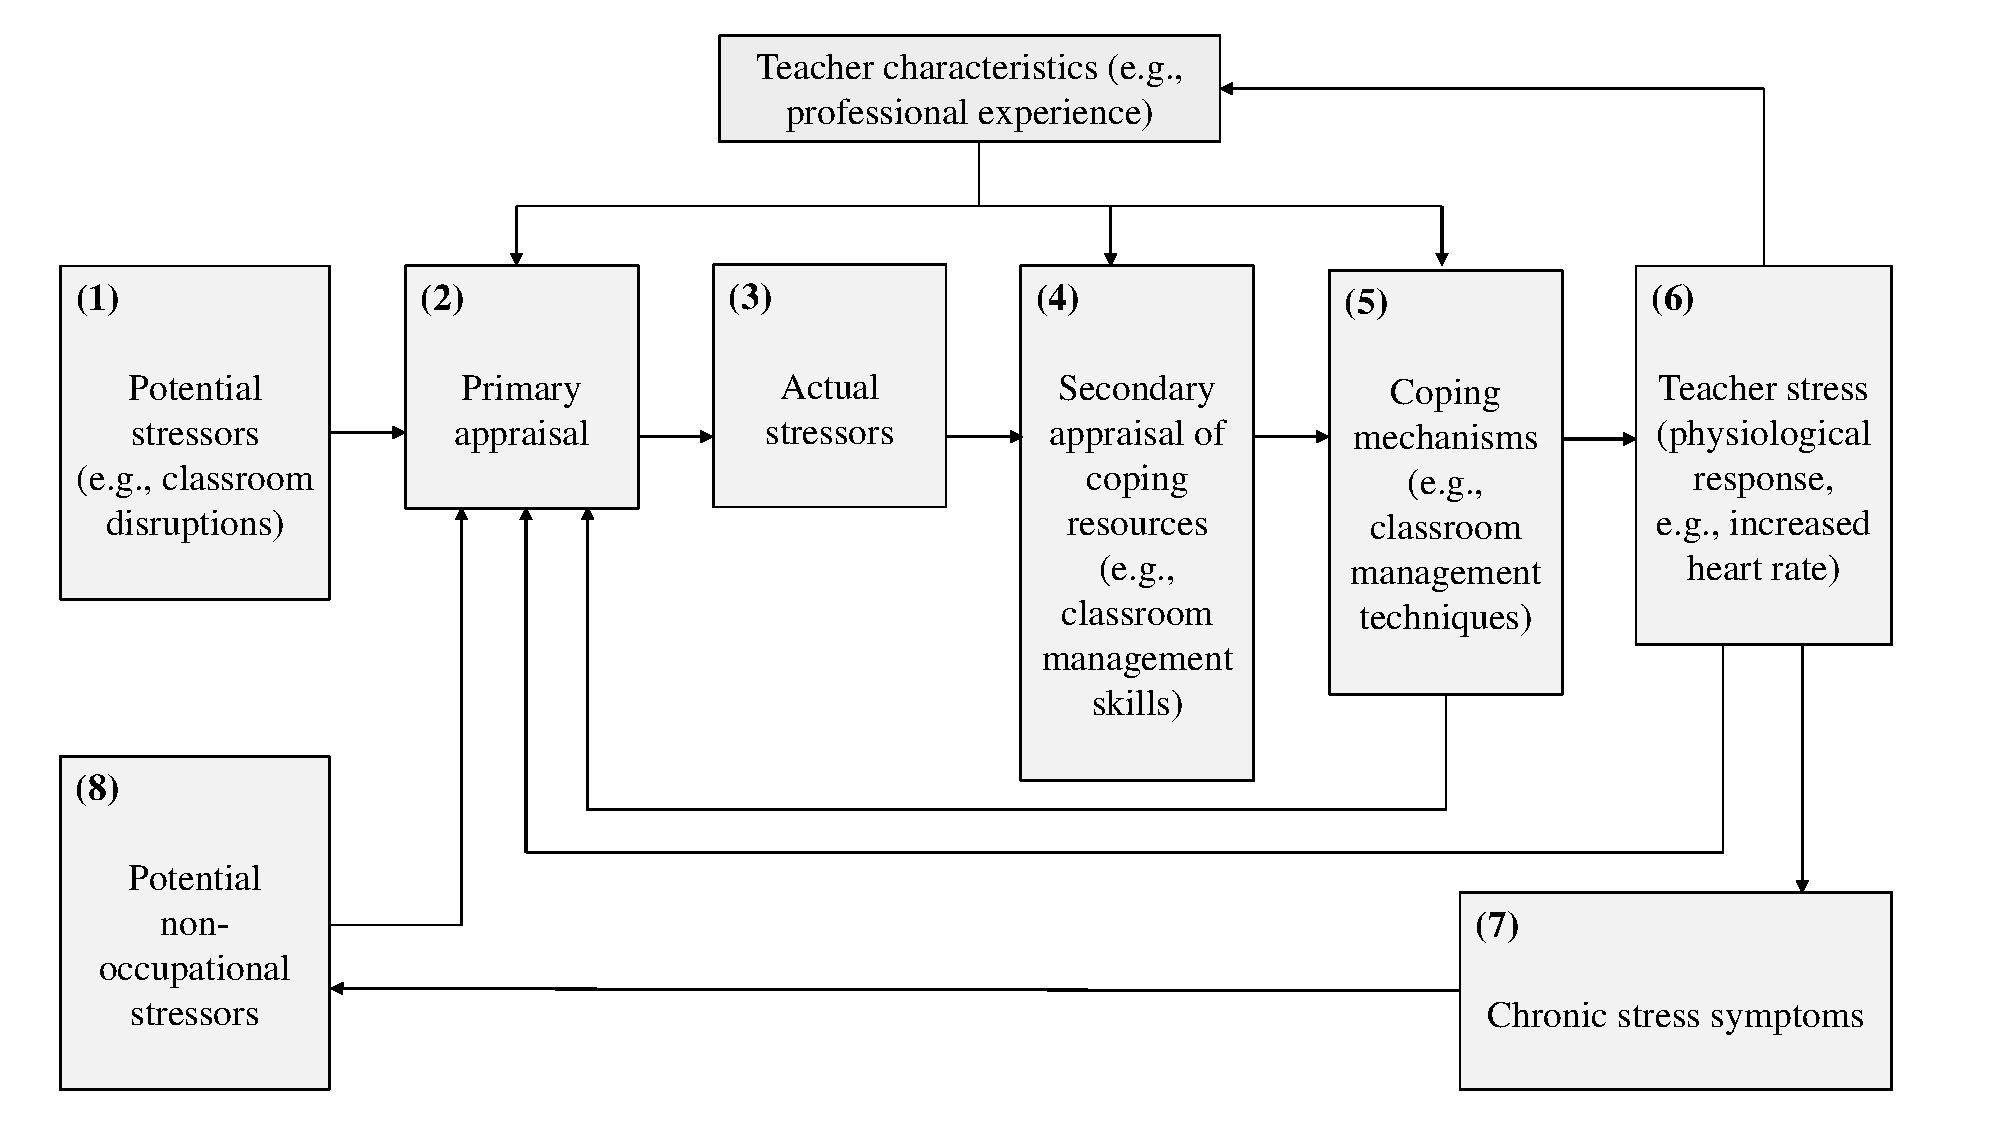
\includegraphics[width=1\textwidth]{images/Model_Teacher_Stress_adapted_new.pdf}
  \caption{A model of teacher stress (adapted from van Dick 2006, p.37, modified by the authors).}
  \label{fig.1}
\end{figure}

\subsection{Present Study}\label{present-study}

The present study aimed to explore the relations between teachers' HR
response, and their subjective appraisals of stress during a
micro-teaching unit, and to relate their self-reported appraisals and
physiological stress responses to their teaching experience. We analyzed
data from in-service and pre-service teachers who participated in a
laboratory study as part of a larger project targeting the development
of classroom management skills. Participants came to the lab
individually and taught a short lesson to a class of three actors (i.e.,
trained student assistants) who performed several typical and possibly
disruptive classroom events. The micro-teaching unit was thus
potentially stressful for the participants. The aims of the present
study were twofold:

\begin{enumerate}
\def\labelenumi{(\arabic{enumi})}
\tightlist
\item
  The first research goal was to investigate whether HR measures
  assessed by a wrist-based fitness tracker were a suitable and
  effective method for mapping teachers' HR over the course of the lab
  study, with a total duration of approximately 2 hours, including
  phases before, during, and after the stressful micro-teaching unit.
\end{enumerate}

Looking at HR measures globally, we expected the participants to show an
initial increase in their HR, followed by a peak during the
micro-teaching unit and a decrease for the remaining phases. In
addition, we examined whether z-standardization of the participants' HR
could serve as a useful method to account for individual differences in
baseline HR: We expected to observe the same trends in both standardized
and non-standardized HR values.

In addition, we selected five representative 10-minute intervals from
the five phases of the lab study (see Fig.\ref{fig.2}) in order to test
the hypotheses that, regarding HR levels, teachers' HR would be the
highest during the micro-teaching unit, compared to all other phases
(Hypothesis 1a), and, regarding HR slopes, that teachers' HR would
increase while they were preparing for teaching (pre-teaching interval),
but decrease in all of the following intervals, i.e.~when they were
habituating to and recovering from the stressful micro-teaching unit
(Hypothesis 1b).

\begin{enumerate}
\def\labelenumi{(\arabic{enumi})}
\setcounter{enumi}{1}
\tightlist
\item
  We further explored whether teaching experience made a difference in
  how teachers' HR reacted to the classroom disruptions. We expected
  more experienced teachers to be less stressed by the classroom events
  (Hypothesis 2a). In addition, we examined the relations between
  teachers' subjective appraisals of the classroom events (specifically,
  the disruptiveness of the events, and their confidence in dealing with
  them) and teachers' HR level, beyond the explanatory power of teaching
  experience. We expected higher HR levels for teachers who felt more
  disrupted, regardless of their teaching experience (Hypothesis 2b),
  and lower HR levels for teachers who felt more confident, regardless
  of teaching experience (Hypothesis 2c). We hypothesized that each of
  the three predictors (\emph{teaching experience, disruption appraisal,
  confidence appraisal}) uniquely contributed to explaining variance in
  teachers' HR levels (Hypothesis 2d). In addition, we exploratively ran
  analogous analyses for the \emph{changes} in HR (i.e., slopes).
\end{enumerate}

\section{Method}\label{method}

\subsection{Participants}\label{participants}

The sample consisted of \(N\) = 84 pre- and in-service teachers from
Germany, who were recruited via personal contacts, email lists, and
flyers. The data of three participants was lost due to failed data
transmission, yielding an analysis sample of \(n_{total}\) = 81
(\(n_{total}\) = 52 women, \(n_{total}\) = 29 men), including 40
pre-service and 41 in-service teachers. Participants had a mean age of
30.95 years (\(SD\) = 10.90; range: 19-60) and an average teaching
experience of 5.64 years (\(SD\) = 9.46; range: 0-37).

\subsection{Setting and Procedure}\label{setting-and-procedure}

The study was carried out following the ethical standards and the
approval of the University's Institutional Review Board. All
participants were informed in detail about the aims of the study prior
to testing. Participation was voluntary, not incentivized, and only took
place after written consent had been given.

Each participant came to the lab for a period of approximately two hours
in total, and each participant underwent the same phases (see
Fig.\ref{fig.2}): In the \emph{pre-teaching phase}, the experimenter
welcomed the participants and helped them put on the fitness tracker.
This was followed by a warm-up session to familiarize the participants
with the laboratory setting and the class. This phase took about 10-15
minutes and participants spent this time mostly standing or slowly
walking around. During the \emph{teaching phase}, the participants held
their self-prepared micro-teaching unit to a class of three trained
actors who performed nine, potentially disruptive, classroom events
(e.g., chatting with a neighbor, heckling, looking at the phone; see
Tab.\ref{tab_a1} in the supplementary material for an overview and
categorization of all events; and Fig.\ref{fig.a2} in the supplementary
material for a depiction of the laboratory setting of the micro-teaching
unit). The topic and class level of the teaching unit could be freely
chosen by the teachers with the only requirement that the unit had to be
an introductory lesson, and had to consist of supervised individual work
and / or frontal teaching. The micro-teaching unit lasted about 15-20
minutes. Participants spent this time mostly standing or slowly walking
around. While teaching, participants wore eye-tracking glasses, and
their lesson was video-recorded. After having completed the
micro-teaching unit, in the \emph{post-teaching phase}, participants
filled in questionnaires for approximately 10-15 minutes: a brief
computer-based survey of sociodemographic data (e.g., teaching
experience, gender, studied school type, studied school subjects,
extracurricular teaching activities), and a short knowledge test that
was irrelevant to the present study. In the \emph{interview phase},
participants engaged in a Stimulated Recall Interview (SRI). During the
SRI, participants sat in front of a computer monitor and watched the
video of their own lesson from the ego perspective, as recorded through
the eye-tracking glasses. The experimenter stopped the video each time
one of the nine classroom events happened, and asked five open-ended,
and three rating questions per event. Two of the rating questions are
relevant to the present study: the disruption and the confidence
appraisal ratings (see Measures). The interview lasted about 45-60
minutes. Finally, in the \emph{end phase}, participants filled in
another questionnaire irrelevant to the present study, which lasted
about 10-15 minutes. \newpage

\begin{wrapfigure}[36]{r}{0.5\textwidth}
  \centering
  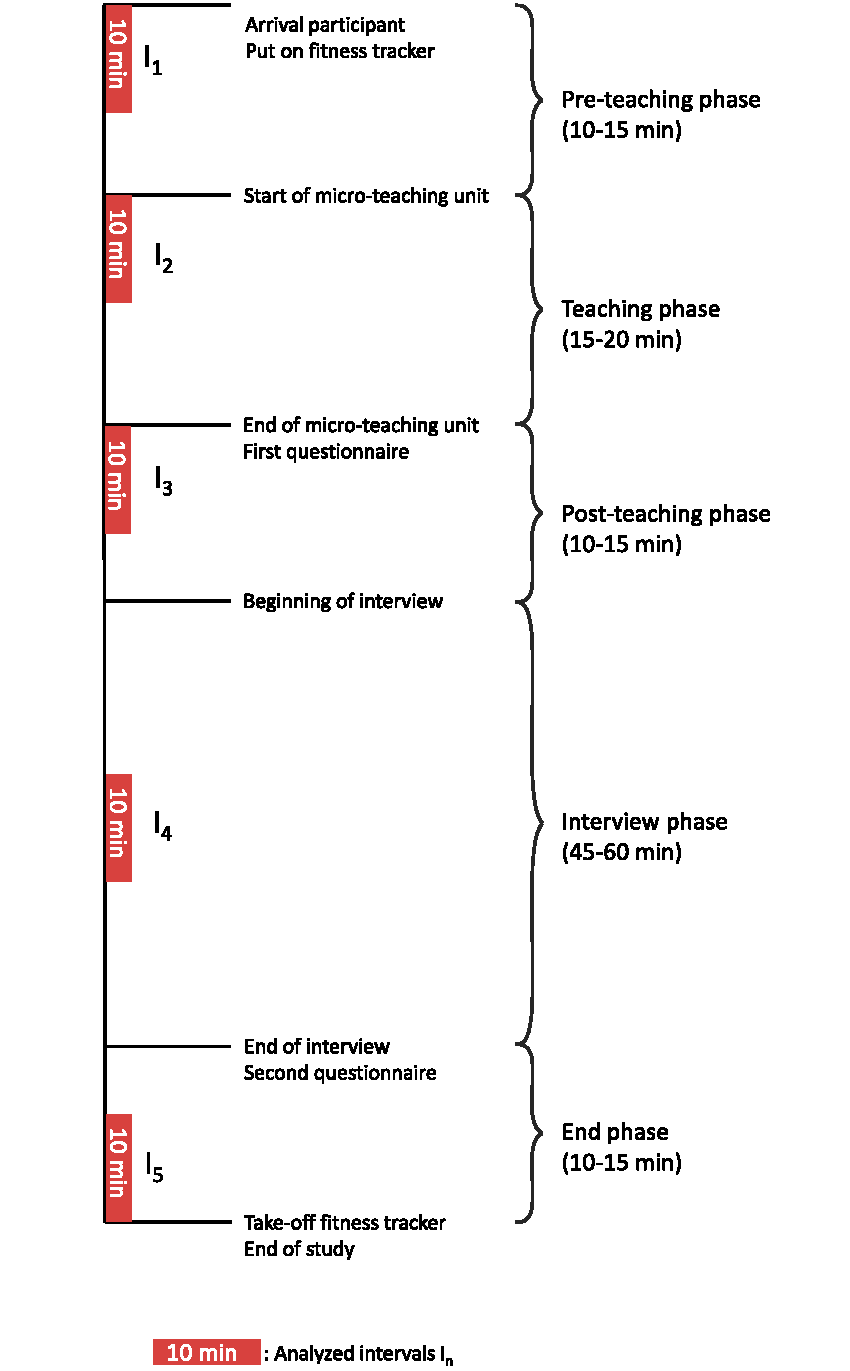
\includegraphics[width=0.5\textwidth]{images/Timeline_smaller.pdf}
  \caption{Procedure of the two-hour-long study consisting of five phases with five representative 10-minute intervals.}
  \label{fig.2}
\end{wrapfigure}

\subsection{Measures}\label{measures}

\subsubsection{Heart Rate Data and Heart Rate
Intervals}\label{heart-rate-data-and-heart-rate-intervals}

To measure teachers' HR, we used the wrist-based fitness tracker Fitbit®
Charge 4. In line with the manufacturer's instructions (Fitbit 2020),
the device was attached to the participants' nondominant hand, a
finger's width above the wrist bone. The tracker works by flashing green
LEDs hundreds of times per second, using light-sensitive photodiodes to
catch the reflected light, to calculate the volume changes in the
capillaries. From this, the tracker calculated the heart beats per
minute. HR measurements were generated at least every 15
seconds\footnote{The fluctuations in the number of seconds in which the
  HR was measured are due to the participants' movements, meaning that
  the device could not measure the HR every second.}. The raw data
contained the estimated HR in BPM for each time stamp. To account for
individual differences in the baseline HR, we also calculated
z-standardized HR values based on individual means, i.e., at the subject
level of \(n\) = 81 participants (standardized HR).

Since we aimed to keep measurement intervals comparable between study
phases, we aggregated HR over a representative 10-minute interval within
each phase (cf.~Fig.\ref{fig.2}). Previous research has indicated that
10-minute intervals are a useful duration for analyzing PPG data (Lu et
al. 2008). The intervals were selected based on the following rules: The
\emph{pre-teaching interval} (\(I_1\)) comprised the first 10 minutes
after the fitness tracker had been put on. The \emph{teaching interval}
(\(I_2\)) started two minutes after the lesson had started. This
interval was of the highest relevance to our study. We explicitly chose
an early 10-minute interval within the teaching phase, as previous
studies revealed that the beginning of a lesson is most demanding and
potentially stressful with regards to teacher-student interaction
(Donker, Van Gog, and Mainhard 2018; Claessens et al. 2017). The
\emph{post-teaching interval} (\(I_3\)) started immediately after the
end of the teaching unit. The \emph{interview interval} (\(I_4\)) was
defined as the mid-10 minutes between the end of the teaching unit and
the time point when the fitness tracker was taken off. All participants
were being interviewed during this interval. The end interval (\(I_5\))
comprised the last 10 minutes before the fitness tracker was taken off.

\subsubsection{Teaching Experience}\label{teaching-experience}

Participants' teaching experience was assessed as a part of their
sociodemographic data. Participants stated their work experience in
years.

\subsubsection{Subjective appraisal of the classroom events and coping
processes}\label{subjective-appraisal-of-the-classroom-events-and-coping-processes}

The subjective disruption and confidence appraisals were assessed during
the SRI on an 11-point rating scale, ranging from 0 (not at all
disrupting/confident) to 10 (extremely disrupting/confident). Ratings
were averaged across the nine classroom events for each participant, as
we were interested in the general stressfulness of the \emph{teaching
phase} for each participant.

\subsection{Data analysis}\label{data-analysis}

We conducted all analyses with R (RStudio Team 2020). Graphics were
created using ggplot2 (Wickham 2016).

To enable visual inspection of HR trends, we displayed smoothed teacher
HR over the course of the recording.\footnote{The curve was smoothed
  using the geom\_smooth() function from the ggplot2 package in R
  (Wickham 2016) based on the smoothing method LOESS (Locally Estimated
  Scatterplot Smoothing). This method fits a polynomial surface
  determined by one or more numerical predictors, using local fitting.}
We visually compared unstandardized and standardized HR trends over the
two-hour recording period.\footnote{Note that the study exceeded the
  planned duration of two hours for a few participants. To avoid
  distortions when mapping the HR over the course of the study (see
  Fig.\ref{fig.3}), the endpoint was set at two hours for all
  participants, even though data from later time points was used in the
  \emph{end interval} for a few participants.} For all further analyses,
we used standardized rather than unstandardized HR values.

We averaged each person's standardized HR over each of the five selected
intervals\footnote{We used the mean standardized HR instead of the mean
  intercept as we wanted to explain the mean HR of the entire intervals
  and not the HR at the very beginning of the interval (\(x\) = 0).},
resulting in one measure per person per interval. To test Hypothesis 1a,
we initially conducted a one-way ANOVA with repeated measures as an
omnibus test and then tested the mean differences between the
\emph{teaching interval} (\(I_2\)) and the other four intervals by
planned contrasts and inspection of effect size \(d\) (Cohen 1988).

For testing Hypothesis 1b, concerning HR changes within each interval,
we first conducted a linear estimation of the increase or decrease in
standardized HR values over time for each participant. To this end, we
used fixed intercept fixed slope regression models (Gelman and Hill
2006) for each interval to estimate intercepts and linear slopes for
each individual, which were then averaged across individuals.\footnote{Although
  this procedure does not account for nonmonotonic progressions in
  individual HR, a graphical evaluation revealed that the linear
  estimates corresponded well to the majority of the cases (see
  Fig.\ref{fig.a3} to \ref{fig.a7} in the supplementary material).} We
tested Hypothesis 1b based on the unstandardized estimates of mean
slopes (one estimate per participant per interval).

Addressing our second research goal, we ran linear regression analysis
with teaching experience and subjective appraisals as predictors. To
test Hypothesis 2a, we examined the effect of teaching experience on
participants' HR levels (i.e., mean standardized HR) for each of the
five intervals, using linear regression models with teaching experience
as the sole predictor. To test Hypotheses 2b and 2c, we separately
augmented the model by either teachers' disruption appraisal (Hypothesis
2b) or confidence appraisal (Hypothesis 2c) as predictors, while
controlling for teaching experience. To test Hypothesis 2d, we examined
the effects of all three predictors in one regression model.
Furthermore, we repeated these steps to explore the effects of teaching
experience and subjective appraisals on \emph{changes} in teachers' HR
(i.e., mean slopes).\footnote{Please note: HR levels and changes were
  not regressed on the disruption and confidence appraisals in the
  \emph{pre-teaching interval} (\(I_1\)), because the appraised
  classroom events had not yet taken place in that phase.}

\section{Results}\label{results}

\subsection{Mapping teachers' HR over the course of the study
phases}\label{mapping-teachers-hr-over-the-course-of-the-study-phases}

Means, standard deviations, and range of teachers' unstandardized and
standardized HR for the entire study period, and for the five intervals,
are shown in Tab.\ref{tab_1}. Fig.\ref{fig.3} displays the
unstandardized and standardized HR trends, respectively, over the course
of the entire study period. HR initially increased, peaked, and then
decreased, with the unstandardized and standardized HR graphs showing
high similarity. Thus, for all further analyses, we used participants'
standardized HR values.

Fig.\ref{fig.4} shows the distribution of teachers' mean standardized HR
for the five intervals. Repeated measures ANOVA revealed significant
differences in mean standardized HR between intervals,
\(F(4, 400) = 260.62\), \(p < .05\), \(d = 1.60\) (large effect).
Planned contrasts indicated that, as hypothesized (Hypothesis 1a), mean
standardized HR was significantly higher in the \emph{teaching interval}
(\(I_2\)) than in all other intervals, specifically, the
\emph{pre-teaching interval} (\(I_1\); \(t(400) = -10.08\), \(p < .05\),
\(d = 1.034\); large effect), the post-teaching interval (\(I_3\);
\(t(400) = -6.94\), \(p < .05\), \(d = 1.37\); large effect), the
interview interval (\(I_4\); \(t(400) = 15.00\), \(p < .05\),
\(d = 3.29\); large effect), and the end interval (\(I_5\));
\(t(400) = 22.54\), \(p < .05\), \(d = 4.64\); large effect).

Next, we examined HR changes (i.e., mean slopes) within each interval to
test the hypothesis that HR increased during the \emph{pre-teaching
phase} and decreased during all other phases (Hypothesis 1b). The mean
intercepts and mean slopes, complemented by their standard deviations
for each interval, are shown in Tab.\ref{tab_2}. The mean slope of the
\emph{pre-teaching interval} (\(I_1\)) was significantly positive,
indicating an increase in HR, as hypothesized. Further, the mean slopes
of the \emph{teaching interval} (\(I_2\)), \emph{post-teaching interval}
(\(I_3\)), and \emph{interview interval} (\(I_4\)) were significantly
negative, indicating a decrease in HR. For the last interval, the
\emph{end interval} (\(I_5\)), the mean slope was negative, but did not
differ significantly from zero.

\renewcommand{\arraystretch}{1.5}

\begin{table}[ht]
    \centering
    \begin{tabularx}{\textwidth}{lXXXXX}
        \toprule
        Interval & \textit{M} HR & \textit{SD} HR & Min & Max \\
        \midrule
        Overall Course of 2h & 90.09/0.04\footnotemark[12] & 15.76/0.991 & 51/-4.03 & 164/4.56 \\
        Pre-teaching interval (I$_1$) & 96.28/0.48 & 14.11/0.88 & 56/-3.56 & 139/3.24 \\
        Teaching interval (I$_2$) & 100.80/0.85 & 16.23/0.77 & 63/-2.18 & 164/4.37 \\
        Post-teaching interval (I$_3$) & 93.61/0.27 & 14.01/0.76 & 60/-2.17 & 150/3.06 \\
        Interview interval (I$_4$) & 82.32/-0.72 & 11.85/0.74 & 51/-2.51 & 132/4.39 \\
        End interval (I$_5$) & 77.95/-1.07 & 11.14/0.57 & 50\footnotemark[13]/-2.68 & 120/2.96 \\
        \bottomrule
    \end{tabularx}
    \caption{Mean HR (\textit{M}), standard deviations HR (\textit{SD}), and range of teachers’ HR over the course of the entire study and the five intervals (unstandardized in BPM/z-standardized).}
    \label{tab_1}

    
\end{table}
 \footnotetext[12]{Please note that standardized \textit{M} and \textit{SD} of the overall course were not exactly 0 and 1 due to rounding differences.}
 \footnotetext[13]{Deviations of the minimum values in the overall course vs. the \textit{end interval} ($I_5$) are due to data of a few participants who needed more than two hours to finish the study.}

\renewcommand{\arraystretch}{1.5} 

\begin{table}[ht]
    \centering
    \begin{tabularx}{\textwidth}{lXXXXXX}
        \toprule
        Interval  & \multicolumn{2}{c}{\textit{M} (\textit{SD})} & \multicolumn{2}{c}{$p$} \\ & Intercept & Slope & Intercept & Slope \\
        \midrule
        Pre-teaching interval (I$_1$) & 0.052 (0.820) & 0.085 (0.133) & .57 & $< .05$ \\
        Teaching interval (I$_2$) & 1.025 (0.690) & -0.039 (0.108) & $< .05$ & $< .05$ \\
        Post-teaching interval (I$_3$) & 0.549 (0.547) & -0.060 (0.101) & $< .05$ & $< .05$ \\
        Interview interval (I$_4$) & -0.617 (0.614) & -0.022 (0.070) & $< .05$ & $< .05$ \\
        End interval (I$_5$) & -1.004 (0.500) & -0.012 (0.074) & $< .05$ & .14 \\
        \bottomrule
    \end{tabularx}
    \caption{Analysis (\textit{M, SD, p}-values) for the mean intercepts and the mean slopes for the five intervals.}
    \label{tab_2}
\end{table}

\begin{figure}[H]
  \centering
  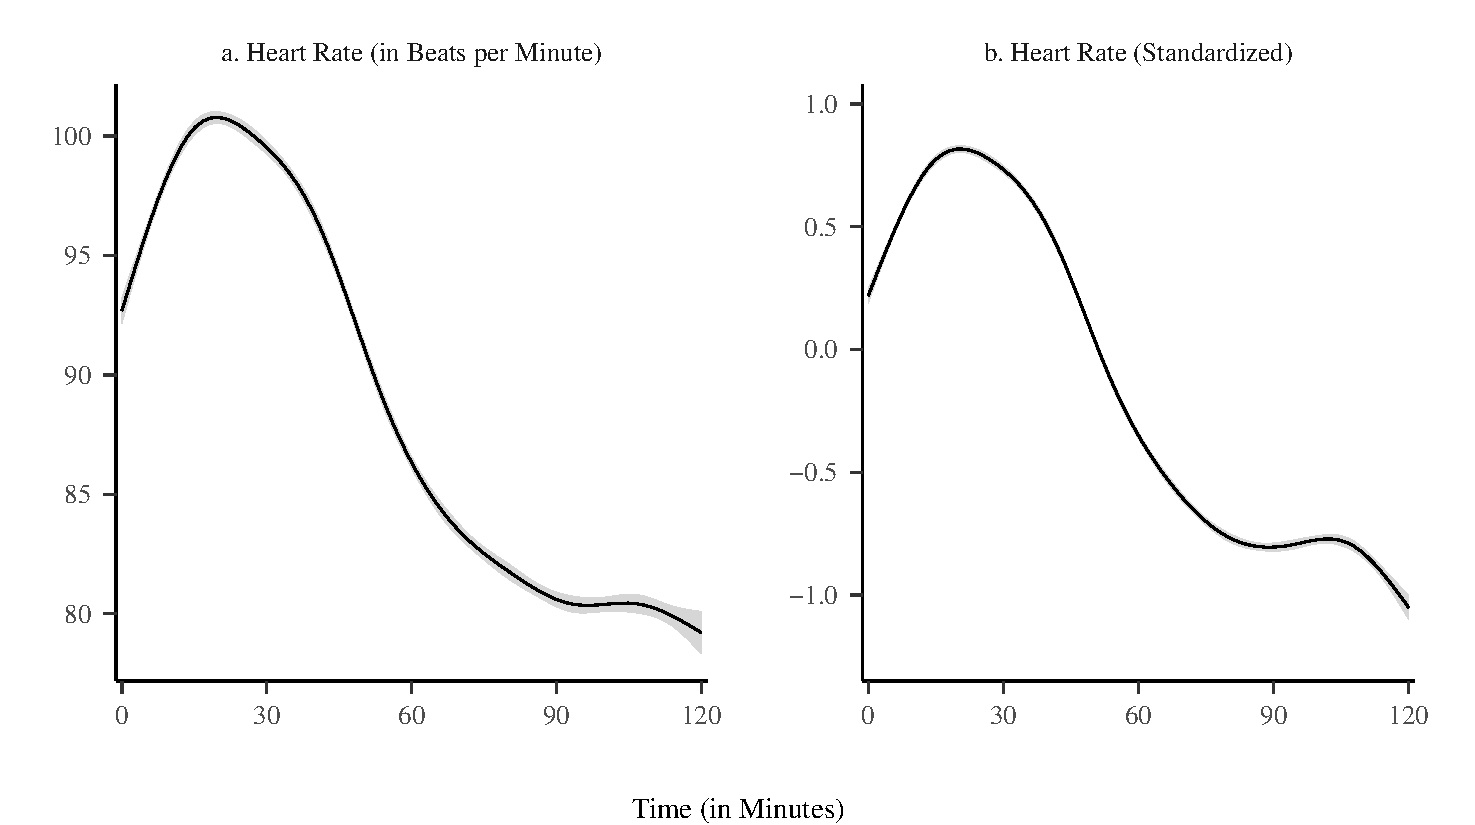
\includegraphics[width=1\textwidth]{plots_publication/loess_plot_std_unstd_new.pdf}
  \caption{Overall course of the HR with the unstandardized HR in BPM shown in Fig.3a. and the z-standardized HR shown in Fig.3b. for the planned 2-hour study.}
  \label{fig.3}
\end{figure}

\begin{figure}[H]
  \centering
  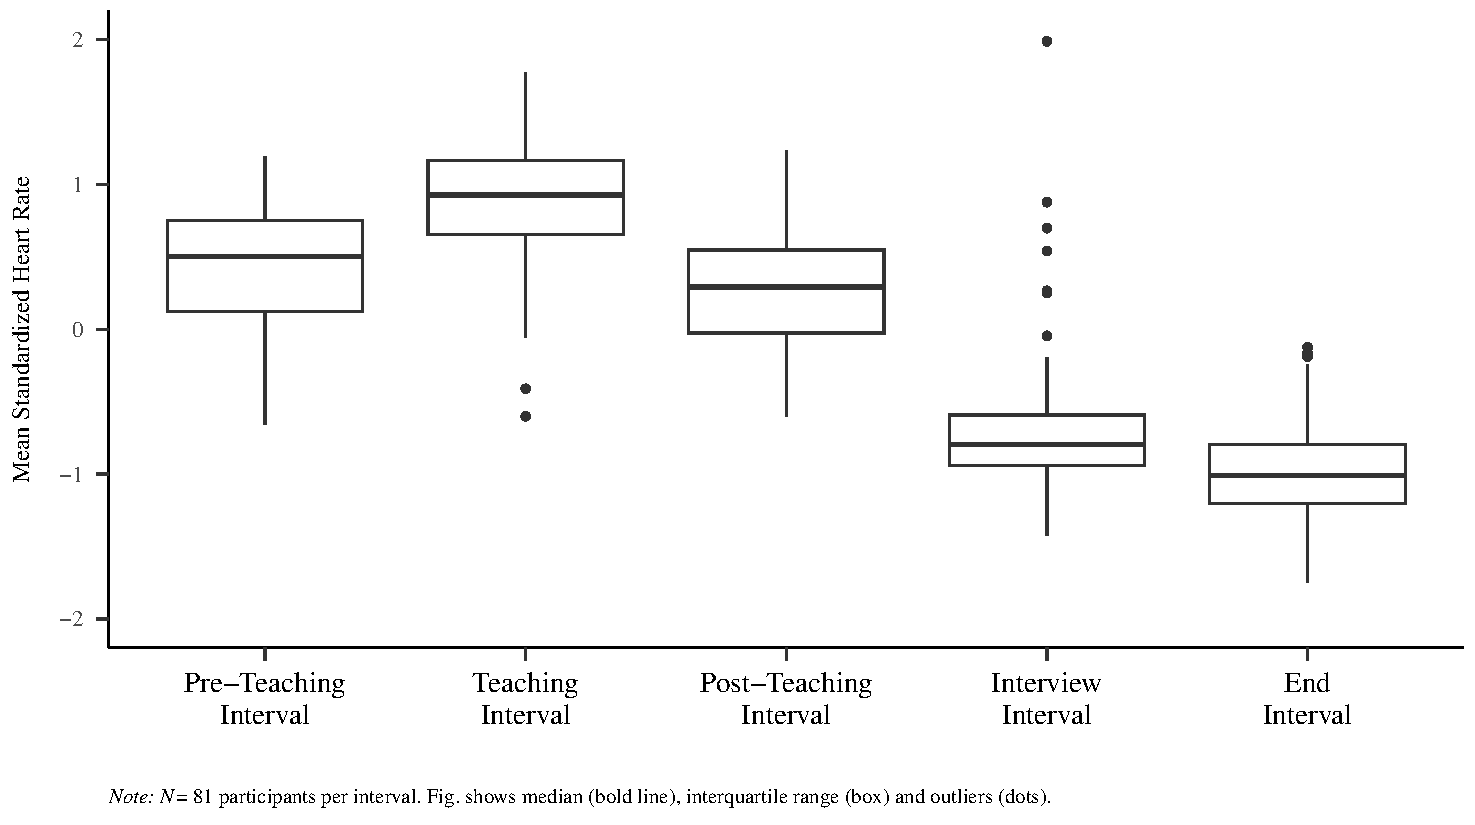
\includegraphics[width=1\textwidth]{plots_publication/box_plot.pdf}
  \caption{Distribution of the standardized heart rate means in the five intervals.}
  \label{fig.4}
\end{figure}

\subsection{Predicting mean standardized HR and mean
slopes}\label{predicting-mean-standardized-hr-and-mean-slopes}

Tab.\ref{tab_3} shows the raw correlations among mean standardized
HR/mean slopes (see Tab.\ref{tab_2} for means and standard deviations),
teaching experience (\(M = 5.64\), \(SD = 9.46\)), disruption appraisal
(\(M = 5.19\), \(SD = 2.87\)), and confidence appraisal (\(M = 7.81\),
\(SD = 1.97\)). With a few notable exceptions, correlations with HR
measures were mostly very small and statistically non-significant
(Tab.\ref{tab_3}). Correlations between teaching experience and
appraisals (not shown in Tab.\ref{tab_3}) were substantial: more
experienced teachers gave lower disruption appraisals (\(r = -.36\)),
and higher confidence appraisals (\(r = .44\)). Moreover, the two
appraisal variables were negatively correlated (\(r = -.37\)).

Tab.\ref{tab_4} shows the results of the regression analyses. Teaching
experience significantly predicted mean standardized HR only in the
\emph{interview interval} (Tab.\ref{tab_4}, \emph{interview interval},
Model 1), indicating a higher mean standardized HR for teachers with
more teaching experience. This relationship is, in fact, in the opposite
direction as predicted by Hypothesis 2a. Neither adding disruption
appraisal (Hypothesis 2b) nor adding confidence appraisal (Hypothesis
2c) increased the amount of explained variance to a statistically
significant extent.

When considering the effects of the three predictors in concert
(Hypothesis 2d), mean standardized HR was significantly predicted only
by disruption appraisal, and only in the \emph{post-teaching interval}
(Tab.\ref{tab_4}, \emph{post-teaching interval}, Model 4), indicating a
higher mean standardized HR for teachers who felt more disrupted by the
classroom events, when controlling for the other variables.

Concerning the explorative investigation of the effects of teaching
experience and subjective appraisals on \emph{changes} (i.e., mean
slopes) in teachers' HR, teaching experience significantly predicted the
mean slope in the \emph{pre-teaching interval} (Tab.\ref{tab_4},
Pre-teaching interval, Model 1), indicating a less steep HR increase in
teachers with more teaching experience. For all other intervals, no
variable had significant predictive value.

\renewcommand{\arraystretch}{1.5}

\begin{table}[h]
    \centering
    \begin{tabularx}{\textwidth}{lccccc}
        \toprule
        Variable & Pre-teaching & Teaching & Post-teaching & Interview & End \\
        & interval & interval & interval & interval & interval \\
        \midrule
        Teaching Experience & $- .17/ - .27^*$ & .11/-.02 & $- .04/-.03$ & $.24^*/-.20$ & .04/.11 \\
        Disruption Appraisal & $- .01/.16$ & $- .20/.08$ & .20/$- .14$ & $- .13/.01$ & .04/.12 \\
        Confidence Appraisal & $- .10/ - .18$ & .06/.09 & .04/$- .03$ & .09/$- .19$ & $- .07/.13$ \\
        \bottomrule \\
          \textit{Note. *} $p < .05$.
    \end{tabularx}
    \caption{Correlations between mean standardized HR/mean slopes and the predictor variables of teaching experience, disruption appraisal, and confidence appraisal for the five intervals.}
    \label{tab_3}
\end{table}

\newpage

\begin{landscape}

\setlength{\LTleft}{0pt}
\setlength{\LTright}{0pt}

\begin{longtable}{@{\extracolsep{\fill}} p{1.8cm} p{1cm} p{1cm} p{1cm} p{1cm} p{1cm} p{1cm} p{1cm} p{1cm} p{1cm} p{1cm} p{1cm} p{1cm} p{1cm} p{1cm} p{1cm} p{1cm} @{}}
    
    \toprule
    & \multicolumn{4}{c}{Model 1} & \multicolumn{4}{c}{Model 2} & \multicolumn{4}{c}{Model 3} & \multicolumn{4}{c}{Model 4} \\
    \cmidrule(lr){2-5} \cmidrule(lr){6-9} \cmidrule(lr){10-13} \cmidrule(lr){14-17}
    Dependent \newline variable: & \multicolumn{16}{c}{Mean standardized HR and mean slopes} \\
    \cmidrule(lr){2-17}
    & \multicolumn{2}{c}{Mean std. HR} & \multicolumn{2}{c}{Mean slopes} & \multicolumn{2}{c}{Mean std. HR} & \multicolumn{2}{c}{Mean slopes} & \multicolumn{2}{c}{Mean std. HR} & \multicolumn{2}{c}{Mean slopes} & \multicolumn{2}{c}{Mean std. HR} & \multicolumn{2}{c}{Mean slopes} \\
    & $\beta$ (SE) & $p$ & $\beta$ (SE) & $p$ & $\beta$ (SE) & $p$ & $\beta$ (SE) & $p$ & $\beta$ (SE) & $p$ & $\beta$ (SE) & $p$ & $\beta$ (SE) & $p$ & $\beta$ (SE) & $p$ \\
    \midrule
    \endfirsthead

    \toprule
    & \multicolumn{4}{c}{Model 1} & \multicolumn{4}{c}{Model 2} & \multicolumn{4}{c}{Model 3} & \multicolumn{4}{c}{Model 4} \\
    \cmidrule(lr){2-5} \cmidrule(lr){6-9} \cmidrule(lr){10-13} \cmidrule(lr){14-17}
    Dependent variable: & \multicolumn{16}{c}{Mean standardized HR and mean slopes} \\
    \cmidrule(lr){2-17}
    & $\beta$ (SE) & $p$ & $\beta$ (SE) & $p$ & $\beta$ (SE) & $p$ & $\beta$ (SE) & $p$ & $\beta$ (SE) & $p$ & $\beta$ (SE) & $p$ & $\beta$ (SE) & $p$ & $\beta$ (SE) & $p$ \\
    \midrule
    \endhead

    \bottomrule
    \multicolumn{17}{c}{{Continued on next page}} \\
    \endfoot

    \bottomrule
    \endlastfoot

    Pre-teaching \newline interval ($I_1$) & & & & & & & & & & & & & & & & \\
    Teaching \newline Experience & \begin{tabular}{@{}c@{}}$-.17$\\$(.005)$\end{tabular} & $.12$ & \begin{tabular}{@{}c@{}}$-.27^*$\\$(.002)$\end{tabular} & $<.05$ & & & & & & & & & & & & \\
    R\textsuperscript{2} & $.030$ & & $.071$ & & & & & & & & & & & & & \\
    \midrule
    Teaching \newline interval ($I_2$) & & & & & & & & & & & & & & & & \\
    Teaching \newline Experience & \begin{tabular}{@{}c@{}}$.11$\\$(.002)$\end{tabular} & $.34$ & \begin{tabular}{@{}c@{}}$-.02$\\$(.001)$\end{tabular} & $.83$ & \begin{tabular}{@{}c@{}}$.04$\\$(.005)$\end{tabular} & $.73$ & \begin{tabular}{@{}c@{}}$.01$\\$(.001)$\end{tabular} & $.96$ & \begin{tabular}{@{}c@{}}$.10$\\$(.006)$\end{tabular} & $.42$ & \begin{tabular}{@{}c@{}}$-.08$\\$(.001)$\end{tabular} & $.54$ & \begin{tabular}{@{}c@{}}$.05$\\$(.006)$\end{tabular} & $.67$ & \begin{tabular}{@{}c@{}}$-.05$\\$(.001)$\end{tabular} & $.72$ \\
    Disruption \newline Appraisal & \begin{tabular}{@{}c@{}}$-.18$\\$(.041)$\end{tabular} & $.13$ & \begin{tabular}{@{}c@{}}$.08$\\$(.010)$\end{tabular} & $.50$ & \begin{tabular}{@{}c@{}}$-.19$\\$(.042)$\end{tabular} & $.13$ & \begin{tabular}{@{}c@{}}$.12$\\$(.010)$\end{tabular} & $.34$ \\
    Confidence \newline Appraisal & \begin{tabular}{@{}c@{}}$.01$\\$(.046)$\end{tabular} & $.92$ & \begin{tabular}{@{}c@{}}$.12$\\$(.011)$\end{tabular} & $.34$ & \begin{tabular}{@{}c@{}}$-.04$\\$(.047)$\end{tabular} & $.76$ & \begin{tabular}{@{}c@{}}$.15$\\$(.012)$\end{tabular} & $.24$ \\
    R\textsuperscript{2} & $.012$ & & $.000$ & & $.040$ & & $.015$ & & $.012$ & & $.010$ & & $.042$ & & $.031$ \\
    $\Delta$ R\textsuperscript{2} & & & $.028$ & & $.015$ & & $.000$ & & $.010$ & & $.030$ & & $.031$ \\
    \midrule
    Post-teaching \newline interval ($I_3$) & & & & & & & & & & & & & & & & \\
    Teaching \newline Experience & \begin{tabular}{@{}c@{}}$-.04$\\$(.005)$\end{tabular} & $.70$ & \begin{tabular}{@{}c@{}}$-.03$\\$(.001)$\end{tabular} & $.80$ & \begin{tabular}{@{}c@{}}$.04$\\$(.005)$\end{tabular} & $.76$ & \begin{tabular}{@{}c@{}}$-.09$\\$(.001)$\end{tabular} & $.44$ & \begin{tabular}{@{}c@{}}$-.08$\\$(.006)$\end{tabular} & $.55$ & \begin{tabular}{@{}c@{}}$-.02$\\$(.001)$\end{tabular} & $.89$ & \begin{tabular}{@{}c@{}}$-.01$\\$(.006)$\end{tabular} & $.91$ & \begin{tabular}{@{}c@{}}$-.07$\\$(.001)$\end{tabular} & $.61$ \\
    Disruption \newline Appraisal & \begin{tabular}{@{}c@{}}$.22$\\$(.040)$\end{tabular} & $.07$ & \begin{tabular}{@{}c@{}}$-.18$\\$(.009)$\end{tabular} & $.14$ & \begin{tabular}{@{}c@{}}$.25^*$\\$(.041)$\end{tabular} & $<.05$ & \begin{tabular}{@{}c@{}}$-.20$\\$(.010)$\end{tabular} & $.12$ \\
    Confidence \newline Appraisal & \begin{tabular}{@{}c@{}}$.08$\\$(.045)$\end{tabular} & $.55$ & \begin{tabular}{@{}c@{}}$-.03$\\$(.011)$\end{tabular} & $.83$ & \begin{tabular}{@{}c@{}}$.14$\\$(.046)$\end{tabular} & $.27$ & \begin{tabular}{@{}c@{}}$-.08$\\$(.011)$\end{tabular} & $.54$ \\
    R\textsuperscript{2} & $.002$ & & $.001$ & & $.043$ & & $.020$ & & $.006$ & & $.002$ & & $.058$ & & $.023$ \\
    $\Delta$ R\textsuperscript{2} & & & $.041$ & & $.019$ & & $.004$ & & $.001$ & & $.056$ & & $.022$ \\
    \midrule
    Interview \newline interval ($I_4$) & & & & & & & & & & & & & & & & \\
    Teaching \newline Experience & \begin{tabular}{@{}c@{}}$.24^*$\\$(.006)$\end{tabular} & $<.05$ & \begin{tabular}{@{}c@{}}$-.20$\\$(.001)$\end{tabular} & $.07$ & \begin{tabular}{@{}c@{}}$.22$\\$(.006)$\end{tabular} & $.06$ & \begin{tabular}{@{}c@{}}$-.23$\\$(.001)$\end{tabular} & $.06$ & \begin{tabular}{@{}c@{}}$.25^*$\\$(.006)$\end{tabular} & $<.05$ & \begin{tabular}{@{}c@{}}$-.14$\\$(.001)$\end{tabular} & $.25$ & \begin{tabular}{@{}c@{}}$.23$\\$(.007)$\end{tabular} & $.07$ & \begin{tabular}{@{}c@{}}$-.17$\\$(.001)$\end{tabular} & $.18$ \\
    Disruption \newline Appraisal & \begin{tabular}{@{}c@{}}$-.05$\\$(.045)$\end{tabular} & $.66$ & \begin{tabular}{@{}c@{}}$-.08$\\$(.006)$\end{tabular} & $.52$ & \begin{tabular}{@{}c@{}}$-.06$\\$(.047)$\end{tabular} & $.61$ & \begin{tabular}{@{}c@{}}$-.12$\\$(.007)$\end{tabular} & $.34$ \\
    Confidence \newline Appraisal & \begin{tabular}{@{}c@{}}$-.02$\\$(.050)$\end{tabular} & $.85$ & \begin{tabular}{@{}c@{}}$-.13$\\$(.007)$\end{tabular} & $.29$ & \begin{tabular}{@{}c@{}}$-.04$\\$(.052)$\end{tabular} & $.76$ & \begin{tabular}{@{}c@{}}$-.16$\\$(.007)$\end{tabular} & $.20$ \\
    R\textsuperscript{2} & $.058$ & & $.040$ & & $.060$ & & $.050$ & & $.058$ & & $.054$ & & $.061$ & & $.069$ \\
    $\Delta$ R\textsuperscript{2} & & & $.002$ & & $.010$ & & $.000$ & & $.014$ & & $.003$ & & $.029$ \\
    \midrule
    End \newline interval ($I_5$) & & & & & & & & & & & & & & & & \\
    Teaching \newline Experience & \begin{tabular}{@{}c@{}}$.04$\\$(.004)$\end{tabular} & $.70$ & \begin{tabular}{@{}c@{}}$.11$\\$(.001)$\end{tabular} & $.32$ & \begin{tabular}{@{}c@{}}$.07$\\$(.005)$\end{tabular} & $.58$ & \begin{tabular}{@{}c@{}}$.18$\\$(.001)$\end{tabular} & $.13$ & \begin{tabular}{@{}c@{}}$.09$\\$(.005)$\end{tabular} & $.46$ & \begin{tabular}{@{}c@{}}$.07$\\$(.001)$\end{tabular} & $.58$ & \begin{tabular}{@{}c@{}}$.10$\\$(.005)$\end{tabular} & $.43$ & \begin{tabular}{@{}c@{}}$.12$\\$(.001)$\end{tabular} & $.33$ \\
    Disruption \newline Appraisal & \begin{tabular}{@{}c@{}}$.06$\\$(.035)$\end{tabular} & $.60$ & \begin{tabular}{@{}c@{}}$.19$\\$(.007)$\end{tabular} & $.12$ & \begin{tabular}{@{}c@{}}$.04$\\$(.037)$\end{tabular} & $.76$ & \begin{tabular}{@{}c@{}}$.23$\\$(.007)$\end{tabular} & $.07$ \\
    Confidence \newline Appraisal & \begin{tabular}{@{}c@{}}$-.11$\\$(.039)$\end{tabular} & $.38$ & \begin{tabular}{@{}c@{}}$.10$\\$(.008)$\end{tabular} & $.43$ & \begin{tabular}{@{}c@{}}$-.10$\\$(.041)$\end{tabular} & $.44$ & \begin{tabular}{@{}c@{}}$.16$\\$(.008)$\end{tabular} & $.22$ \\
    R\textsuperscript{2} & $.002$ & & $.013$ & & $.005$ & & $.053$ & & $.012$ & & $.025$ & & $.013$ & & $.078$ \\
    $\Delta$ R\textsuperscript{2} & & & $.003$ & & $.040$ & & $.010$ & & $.012$ & & $.011$ & & $.065$ \\
    \label{tab_4}
\end{longtable}
    \captionof{table}{Standardized regression coefficients of mean standardized heart rate and mean slopes predicted by teaching experience, disruption appraisal, and confidence appraisal for the five intervals.}
\begin{tablenotes}
\footnotesize
\item \textit{Note.} In Model 1, mean standardized HR and mean slopes were predicted only by teaching experience. In Model 2, solely disruption appraisal was added to teaching experience as a predictor. In Model 3, solely confidence appraisal was added to teaching experience as a predictor. In Model 4, all three predictors were considered in concert. * $p < .05$.
\end{tablenotes}
\end{landscape}

\section{Discussion}\label{discussion}

\subsection{Key findings}\label{key-findings}

Overall, our findings indicate that wrist-worn fitness trackers are a
useful tool for tracking teachers' HR and identifying stressful periods
during teaching. Using HR data from a commercially available and
relatively low-cost Fitbit® fitness tracker, we were able to map
teachers' HR before, during, and after a stressful micro-teaching unit,
with HR increasing in preparation for teaching, peaking during the
teaching phase, and decreasing afterward.

These findings are in line with prior studies showing that teachers' HR
varies depending on their activities and encountered stressors with
increases during phases where teachers are in an exposed position
(Sperka and Kittler 1995; Scheuch and Knothe 1997; Donker, Van Gog, and
Mainhard 2018; Junker, Donker, and Mainhard 2021), as well as with
findings showing how HR changes align with activating events and
stress-inducing tasks (Darnell and Krieg 2019; Chalmers et al. 2021).

Building on the model of teacher stress (Kyriacou and Sutcliffe (1978),
see Fig.\ref{fig.2}), we had hypothesized that more experienced
teachers, with better classroom management skills at their disposal,
experience less physiological stress when dealing with classroom
disruptions. Contrary to our expectations, we found no buffering effect
of teaching experience on teachers' HR, i.e., more experienced teachers
did not show lower mean standardized HR during the stressful teaching
phase than less experienced teachers. Rather, at least descriptively, we
observed the opposite trend. There are several possible explanations for
this finding. First, teaching experience is inherently confounded with
age (the two variables correlated at \(r = .94\) in our sample), and age
has been shown to affect indicators of cardiovascular reactivity in
various ways (Uchino, Birmingham, and Berg 2010). However, to avoid this
kind of confounding influence, we had used not raw BPM but rather
standardized mean HR for all our analyses, thus controlling at least for
inter-individual differences in mean HR. Second, as research on teacher
professionalization has repeatedly shown, professional experience is not
a guarantee for higher professional knowledge and skills (Kirschner et
al. 2016). Rather, honing skills from professional experience
necessitates a deliberate practice of choosing to improve, learning
through experience, and integrating new knowledge into future
performances (Dunn and Shriner 1999). Thus, rather than professional
experience alone, more direct assessments of classroom management
skills, such as objective behavior-based tests, would be a better
indicator of expertise that future studies could explore. Finally, and
most importantly, the highly controlled teaching situation that we
created in the lab might not have provided sufficient resemblance to the
expert teachers' working conditions to let them effectively use their
coping resources. In other words, since the situation was unfamiliar to
both experienced and unexperienced teachers, their stress levels might
have been more similar than they would have been in a more authentic
classroom setting.

While we did not find a buffering effect of teaching experience on mean
HR during teaching, we did, however, find a less steep HR increase in
more experienced, compared to less experienced teachers during the
\emph{pre-teaching phase} (\(\beta = -.27\)), i.e., in preparation for
the micro-teaching unit. This finding supports the idea that, even
though teaching experience guarantees neither superior expertise nor
stress resistance, the habits and routines formed by experienced
teachers may at least lead to lower arousal levels (e.g., experienced as
feeling less nervous and tense) when they anticipate potentially
stressful teaching situations.

An interesting observation beyond our hypotheses was that teaching
experience was predictive of HR differences, not during teaching, but in
the \emph{interview phase}: compared to less experienced teachers, more
experienced teachers showed a higher mean standardized HR
(\(\beta = .24\)) and, thus, probably experienced higher levels of
physiological stress during the SRI. One possible explanation for this
finding could again be the higher age of the more experienced teachers,
along with slower recovery from stress in older teachers. For instance,
Ritvanen et al. (2006) observed that, compared to their younger
colleagues, older teachers did not experience a decrease in their HR
during periods of low stress levels, from which they concluded that
recovery from stress was insufficient in the older teachers (Ritvanen et
al. 2006). Alternatively, the finding could also be attributed to the
fact that less experienced teachers, due to their ongoing or only
recently concluded training, may have been more accustomed to reflecting
on their work and receiving feedback as was the case during the SRI,
whereas, these activities were less routine and possibly more
face-threatening for experienced teachers. Therefore, it is possible
that more experienced teachers found the interview itself to be more
stressful and therefore showed a higher mean standardized HR during this
phase.

With regards to the predictive power of teachers' subjective appraisals
of the classroom disruption during teaching, we, first of all, have to
conclude that our hypotheses were not supported, as neither confidence
appraisal nor disruptiveness appraisal showed any notable correlations
with teachers' mean standardized HR or any explanatory power over and
beyond teaching experience. Possibly, teachers' self-reported
appraisals, and their actual physiological stress responses, tap into
quite different phenomena, or at least, quite different aspects of the
multifaceted stress response (Kyriacou and Sutcliffe 1978). In addition,
while HR was assessed online during teaching, self-reported appraisals
were given in retrospect during the SRI, and may be subject to biased
(e.g., self-serving) reporting or simply an inability to recall ones
immediate stress reactions.

On the other hand, when controlling for all other factors, teachers who
reported to have perceived the events as more disruptive showed a higher
HR (\(\beta = .25\)) in the phase immediately following the
micro-teaching unit. This finding would be consistent with the idea that
differences in mean HR, as an indicator of the physiological stress
response, can be linked to the cognitive appraisal of stressors.

\subsection{Limitations and future
directions}\label{limitations-and-future-directions}

While the laboratory setting of the study allowed for a controlled
implementation of stressors and high internal validity, it was not an
authentic classroom environment, raising questions about its external
validity. Most importantly, the teacher and their students did not have
a shared history, and only a very thin basis for establishing a positive
teacher-student relationship, which is a core characteristic of
effective classroom management (Rüedi 2014; Beaty-O'Ferrall, Green, and
Hanna 2010). In addition, the micro-teaching unit was only about 15
minutes long, and thus much shorter than a regular school lesson,
providing less opportunities for experienced teachers to build up an
engaging lesson. Finally, student behavior was scripted, with classroom
disruptions following the experimental schedule, irrelevant of the
behavior of the teacher. Thus, the setting may have masked effects of
teaching experience by providing too little opportunities of experienced
teachers to demonstrate their true classroom management skills, in
particular regarding the prevention of disruptions. In subsequent
studies, it would therefore be insightful to assess teachers' HR in more
authentic classroom settings over a longer period of time (e.g., days,
weeks, or even months). Extended observation of teachers' HR in
authentic classroom settings could reveal how factors such as student
behavior, teaching methods, or organizational and administrative demands
contribute to fluctuations in physiological arousal, uncovering insights
into the sustained physiological demands of teaching that short-term
studies may overlook. Finally, linking actual teacher behavior to
potential stressors (e.g., classroom disruptions, noise level, etc.)
would offer insights into teacher coping strategies and their links with
physiological indicators of stress.

Another limitation concerns the assessment of teachers' HR. While our
results demonstrate the usefulness of drawing upon easily available HR
data from ubiquitous, low-cost, un-intrusive fitness trackers to
estimate teacher stress, there also are shortcomings of this type of
assessment. First, while fitness trackers typically yield HR data, heart
rate variability (HRV) has been demonstrated to be an even more accurate
indicator of stress (Wettstein et al. 2020). While standard fitness
trackers did not provide this measure at the time of our data
collection, more recent products do offer this function. Thus, future
studies might consider assessing HRV instead of HR. Second, we did not
record participants' resting HR, which is generally considered an
important baseline for determining inter- and intrapersonal differences
in cardiovascular health and reactivity (Nanchen 2018; Heneghan,
Venkatraman, and Russell 2019). A clean baseline HR requires a resting
phase without physical movement or emotional stress, ideally fifteen
minutes before the beginning of the activity, which is very difficult to
achieve in practice (Sammito et al. 2015), e.g., when assessing teacher
HR before and during teaching. Thus, our study explored the possibility
of substituting baseline HR measurement via z-standardization within
participants. As a result, the absolute standardized values of each
participant must always be interpreted in the context of the
standardization sample, and thus are less interpretable than individual
BPM values together with a baseline HR. However, for statistical
analyses based on the whole sample, the standardization fulfills the aim
of controlling for differences in individual HR due to, for example,
age-related differences. Finally, depending on the brand and model of
fitness trackers used, the precision of the HR measurement varies.
Research on the reliability of our deployed Fitbit® device has proven
that this brand is generally accurate in controlled settings and for
moderate activity levels (Wallen et al. 2016; Hajj-Boutros et al. 2023;
Fuller et al. 2020; Jo et al. 2016), as in our study. For example, the
Fitbit® fitness tracker has previously shown good HR measurement
accuracy during resting phases (Jo et al. 2016; Muggeridge et al. 2021)
and for activities such as walking, jogging, and running (Hajj-Boutros
et al. 2023). At higher exercise intensities such as cycling, the
Fitbit® tracker may underestimate HR (Thomson et al. 2019; Montoye,
Mitrzyk, and Molesky 2017; Jo et al. 2016; Jachymek et al. 2021) but is
still within an acceptable range according to systematic reviews
(Chevance et al. 2022). Nevertheless, Gagnon et al. (2022) stressed that
Fitbit® trackers cannot replace ECG when precision is paramount. Despite
these considerations, the Fitbit® model appears suitable for our study
purposes, as physical strain was moderate.

Furthermore, while we assessed teachers' appraisals of the stressful
classroom disruptions using a SRI in which they could review the exact
situation, these appraisal ratings were still post-hoc self-reports,
which limits the interpretation of our results. One of the main issues
with post-hoc self-reports is that they rely on the teachers' memories
and subjective interpretations of past events, which may be prone to
various biases such as social desirability (Razavi 2001) or recall
errors (Van den Bergh and Walentynowicz 2016). Moreover, stress is not a
fixed or stable construct; it is a dynamic, constantly evolving
affective response that can vary depending on context, individual
disposition, and prior experiences, making it particularly challenging
to pinpoint valid and reliable process markers for how individuals
appraise stress in real-time (Lazarus 1990). While SRIs provide a more
detailed and reflective understanding of the stressor in question, the
delayed nature of the response makes it difficult to capture the
immediate, in-the-moment appraisal that occurs when the stressful event
actually takes place.

\subsection{Hands-on advice for using wrist-worn fitness trackers for
research}\label{hands-on-advice-for-using-wrist-worn-fitness-trackers-for-research}

For researchers aiming to use fitness trackers to collect data, there
are practical aspects to consider concerning the design, data
collection, and data analysis phases of research projects (for an
additional overview, see Nelson et al. 2020):

\begin{enumerate}
\def\labelenumi{\arabic{enumi})}
\tightlist
\item
  Choosing a suitable model:
\end{enumerate}

Before data collection, researchers need to decide which model of
fitness tracker best suits their research question. One important point
to consider is whether the study will be conducted in the laboratory, in
a clinical environment, or under real-world conditions. Conventional
fitness trackers should not be used if the focus is on measurement
accuracy, such as in medical contexts, as they cannot replace the
accuracy of ECG measurements (Gagnon et al. 2022). Moreover, researchers
should consider that measurement accuracy also depends on the intensity
of the movements performed by the participants during data collection.
Fitbit® fitness trackers, for example, underestimate HR at higher
exercise intensities such as cycling (Thomson et al. 2019; Montoye,
Mitrzyk, and Molesky 2017; Jo et al. 2016; Jachymek et al. 2021). For
reference, the systematic review by Fuller et al. (2020) provides a
detailed overview of studies that used wrist-worn fitness trackers
between 2000 and 2019 and discusses their validity and reliability.
Another point to consider is the price, which at the time of writing
ranged between €30 for the cheapest models and up to €1.700 for medical
wristbands. Currently, models assessing HRV in addition to HR are
becoming more and more affordable and widespread. Still, Fitbit® fitness
trackers might be a good choice for teams operating with moderate
budgets or if larger groups of participants need to be tracked at the
same time. Further, before conducting any study, it should be considered
that the data collected with fitness trackers is health data, and
therefore very sensitive. Researchers have to ensure that their chosen
model of fitness tracker allows them to collect and store data in line
with relevant ethical and legal requirements, for example, guaranteeing
participants' anonymity and secure data storage.

\begin{enumerate}
\def\labelenumi{\arabic{enumi})}
\setcounter{enumi}{1}
\tightlist
\item
  Operating the fitness tracker:
\end{enumerate}

In planning the operation of their chosen model of fitness tracker,
researchers need to specify the circumference and attachment of the
wrist band and the placement of the fitness tracker on participants. In
particular, researchers conducting studies with children should take
into account their smaller wrist size. When putting on a fitness
tracker, attention must also be paid to whether it is attached to the
dominant or non-dominant wrist, as this can influence HR measurements.
Different models of fitness trackers need to be placed differently and
in line with the manufacturer's instructions. It is also important to
check that the battery is fully charged each time, that the latest
software version is loaded, and that the fitness tracker has been
synchronized before recording data to avoid unnecessary loss of data.
Finally, if researchers want to accurately investigate parameters during
specific time intervals, such as HR during lessons versus breaks, it is
crucial to synchronize the fitness tracker with other time-keeping
devices, such as watches. This synchronization allows researchers to
precisely determine the onset and offset of particular activities or
intervals of interest. By aligning the recorded data with specific time
frames, researchers can ensure that the physiological measurements, such
as HR, are accurately associated with the corresponding periods of
interest. This process enhances the validity and reliability of the data
analysis, enabling a more precise examination of variations in
physiological responses across different time intervals.

\begin{enumerate}
\def\labelenumi{\arabic{enumi})}
\setcounter{enumi}{2}
\tightlist
\item
  Extracting and analyzing fitness tracker data:
\end{enumerate}

As far as the procedure for processing the data is concerned,
researchers should ensure that the raw data of the physiological
measurements are available for further analysis. For the Fitbit® HR
measurements, for example, the raw data can be downloaded from a website
in the form of .csv files. However, these must be downloaded as soon as
possible after data collection, as some platforms automatically delete
or archive older data files after a certain period due to policies
regarding data storage and retention. This can result in loss of access
to critical data. Additionally, ensuring that data is collected at the
intended sampling rate is crucial for accurate analysis. For instance,
while our fitness tracker was designed to record HR every 1-5 seconds,
we occasionally observed recordings only every 15 seconds, possibly due
to participant movement and tracker placement.

\subsection{Conclusion}\label{conclusion}

This study investigated whether HR data collected from teacher-worn
fitness trackers are suitable for exploring links between HR, subjective
stressor appraisal, and individual teaching experience, to achieve a
more profound comprehension of teacher stress. Results suggest that the
widespread availability of HR data from wearable fitness trackers,
moving ``from heartbeat to data'', presents opportunities both to
teachers for self-monitoring stress levels, and to researchers for
assessing physiological indicators of stress. For example, using fitness
trackers could enable teachers to strengthen their self-awareness in
stressful situations and allow for early self-intervention such as
mindfulness techniques (e.g., deep breathing or body scans; Agyapong et
al. (2023)). Integrating fitness trackers into teacher training and
everyday practice could offer an affordable and practical method for
assessing and managing teacher stress. In teacher training as well as in
research, triangulating data from fitness trackers, lesson videos, and
interviews could provide teachers with insights into their own stress
management, and foster the implementation of effective stress and
classroom management strategies. Taken together, our findings cater to
Wettstein et al. (2021) call for the use of ambulatory assessment
methods, particularly in the context of classroom disruptions, for
gaining a deeper understanding of teacher stress and its impact on both
psychological and physiological variables.

In summary, our study contributes to the understanding of stress in
educational settings and underscores the potential of wearable fitness
trackers in advancing research on teacher well-being. By harnessing the
power of wearable technology, we can provide teachers with the tools
needed to better understand and manage their stress, ultimately
enhancing their overall well-being.

\newpage

\appendix
\section*{Appendix}

\setcounter{figure}{0}  % Reset figure numbering

\setcounter{table}{0}

\renewcommand{\thefigure}{A\arabic{figure}}  % Figures labeled A1, A2, etc.

\renewcommand{\thetable}{A\arabic{table}}

\renewcommand{\arraystretch}{1.5}

\begin{table}[ht]
    \centering
    \begin{tabularx}{\textwidth}{XXX}
        \toprule
        Verbal disruptions & Physical disruptions & Lack of eagerness to learn \\
        \midrule
        Heckling & Clicking pen & Looking at phone \\
        Chatting & Snipping hands & Drawing \\
        Whispering & Drumming hands & Head on table \\
        \bottomrule
    \end{tabularx}
    \caption{Classification of nine, typical classroom disruptions according to \cite{lohmann2003schulern} performed in the micro-teaching unit by actors.}
    \label{tab_a1}
\end{table}

\begin{figure}[htbp]
  \centering
  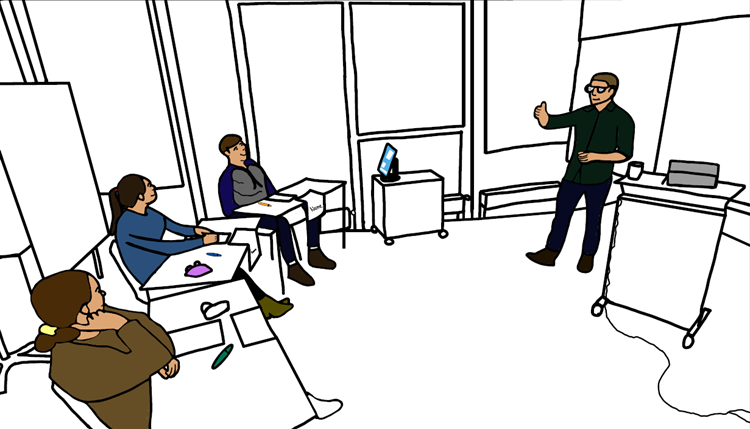
\includegraphics[width=0.45\textwidth]{appendix_figure1.png}
  \caption*{\textit{Note.} The setting included three actors as the class (left) and a teacher (participant, right).}
  \caption{Laboratory setting of the micro-teaching unit.}
  \label{fig.a1}
\end{figure}

\begin{figure}[htbp]
  \centering
  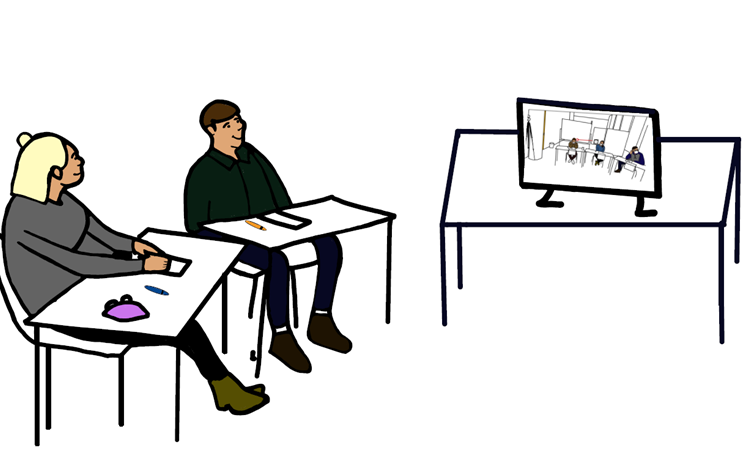
\includegraphics[width=0.45\textwidth]{appendix_figure2.png}
  \caption*{\textit{Note.} The experimenter and participant watched the previously taught micro-teaching unit on video.}
  \centering\caption{Laboratory setting of the interview.}
  \label{fig.a2}
\end{figure}

\begin{figure}[htbp]
  \centering
  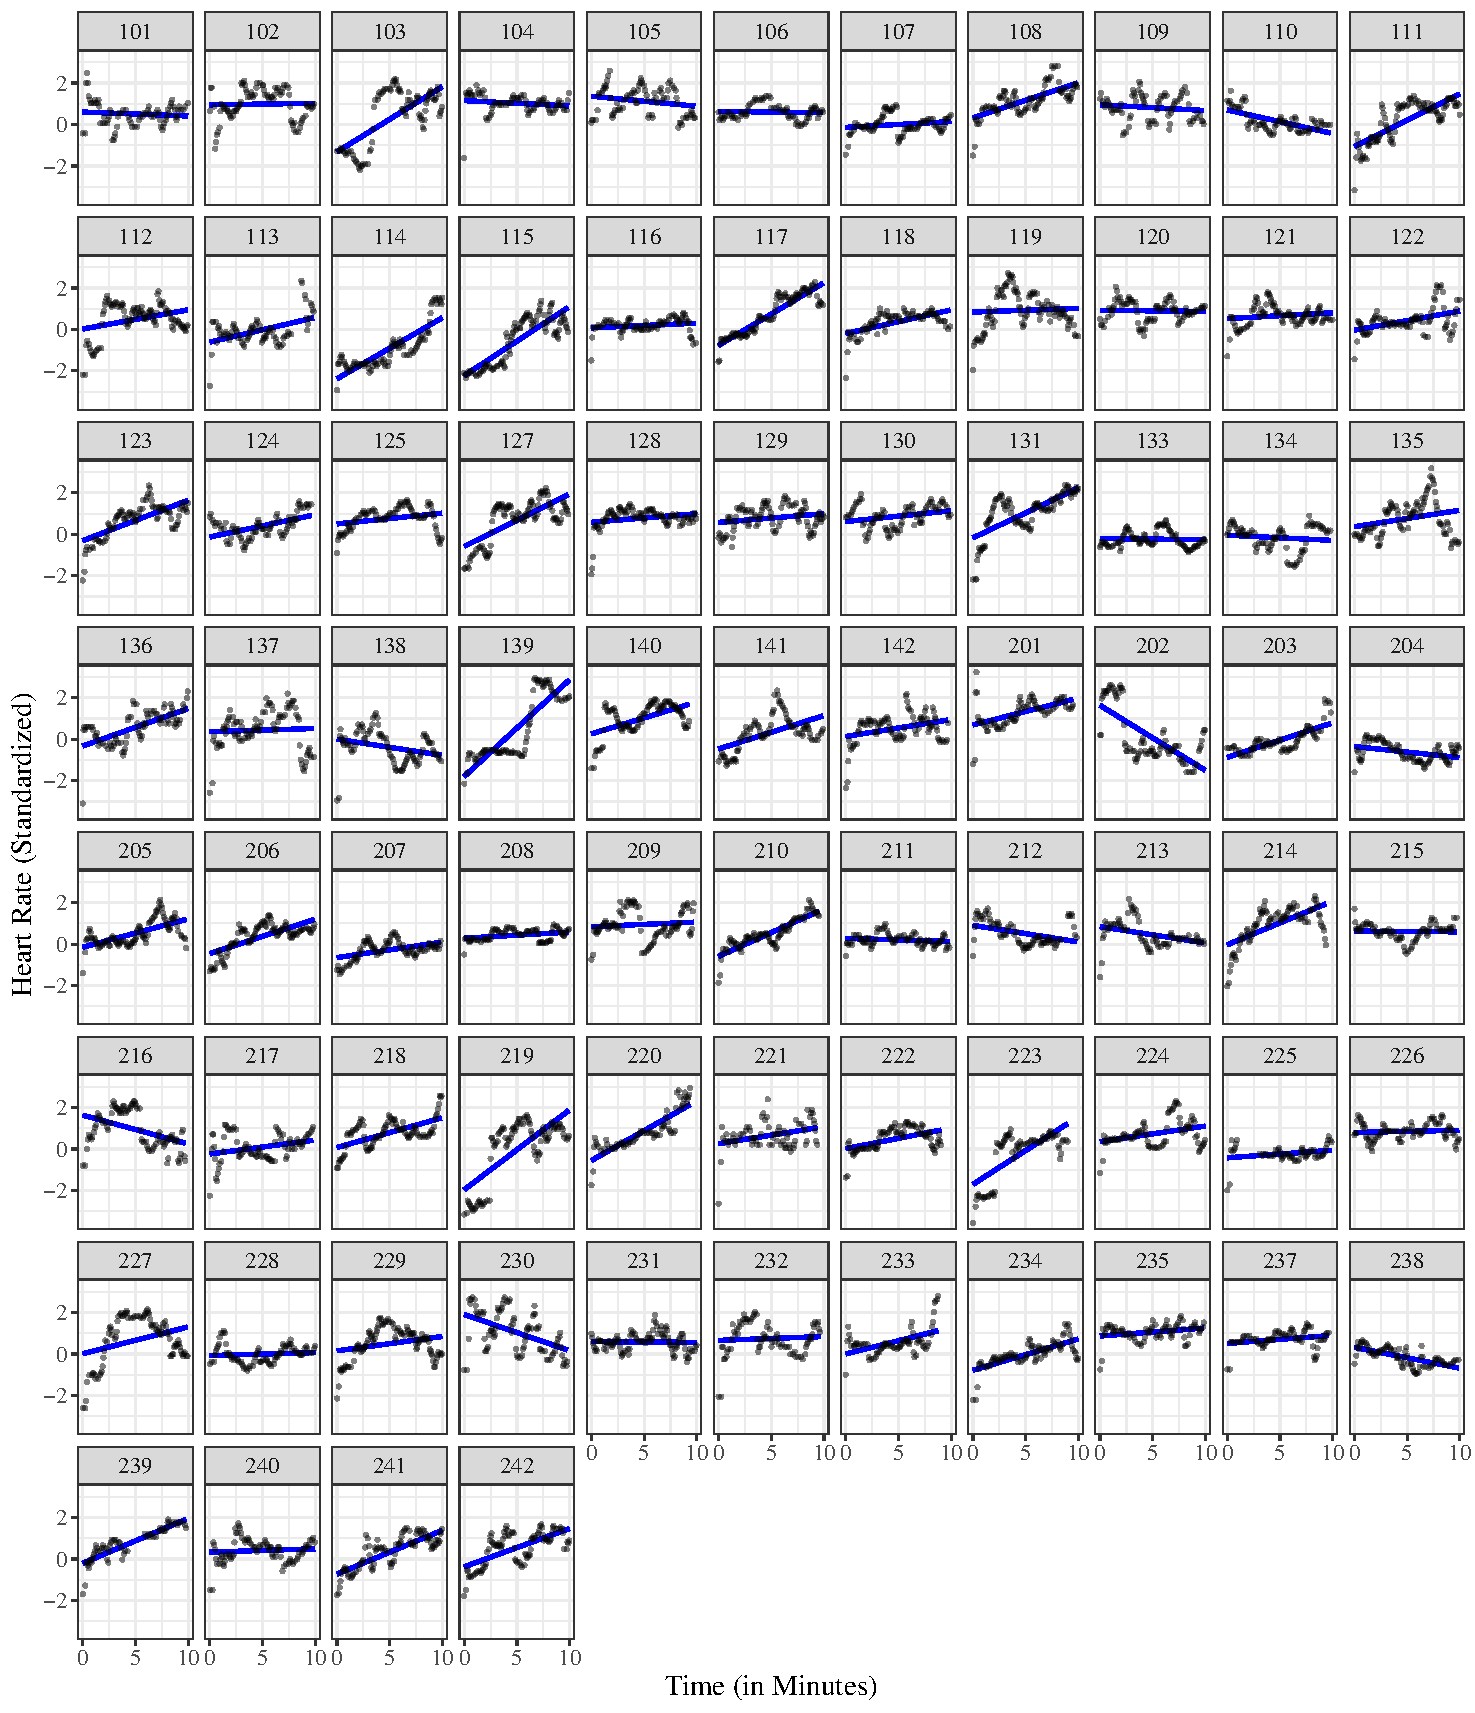
\includegraphics[width=1\textwidth]{plots_publication/plot_preparation_appendix.pdf}
  \caption{Linear estimation of individual HR changes over time during the preparation phase for $N$ = 81 participants. Each plot illustrates the mean standardized HR values (y-axis) across 10 minutes (x-axis), with the black dots representing observed HR data points and the blue line showing the estimated linear trend.}
  \label{fig.a3}
\end{figure}

\begin{figure}[htbp]
  \centering
  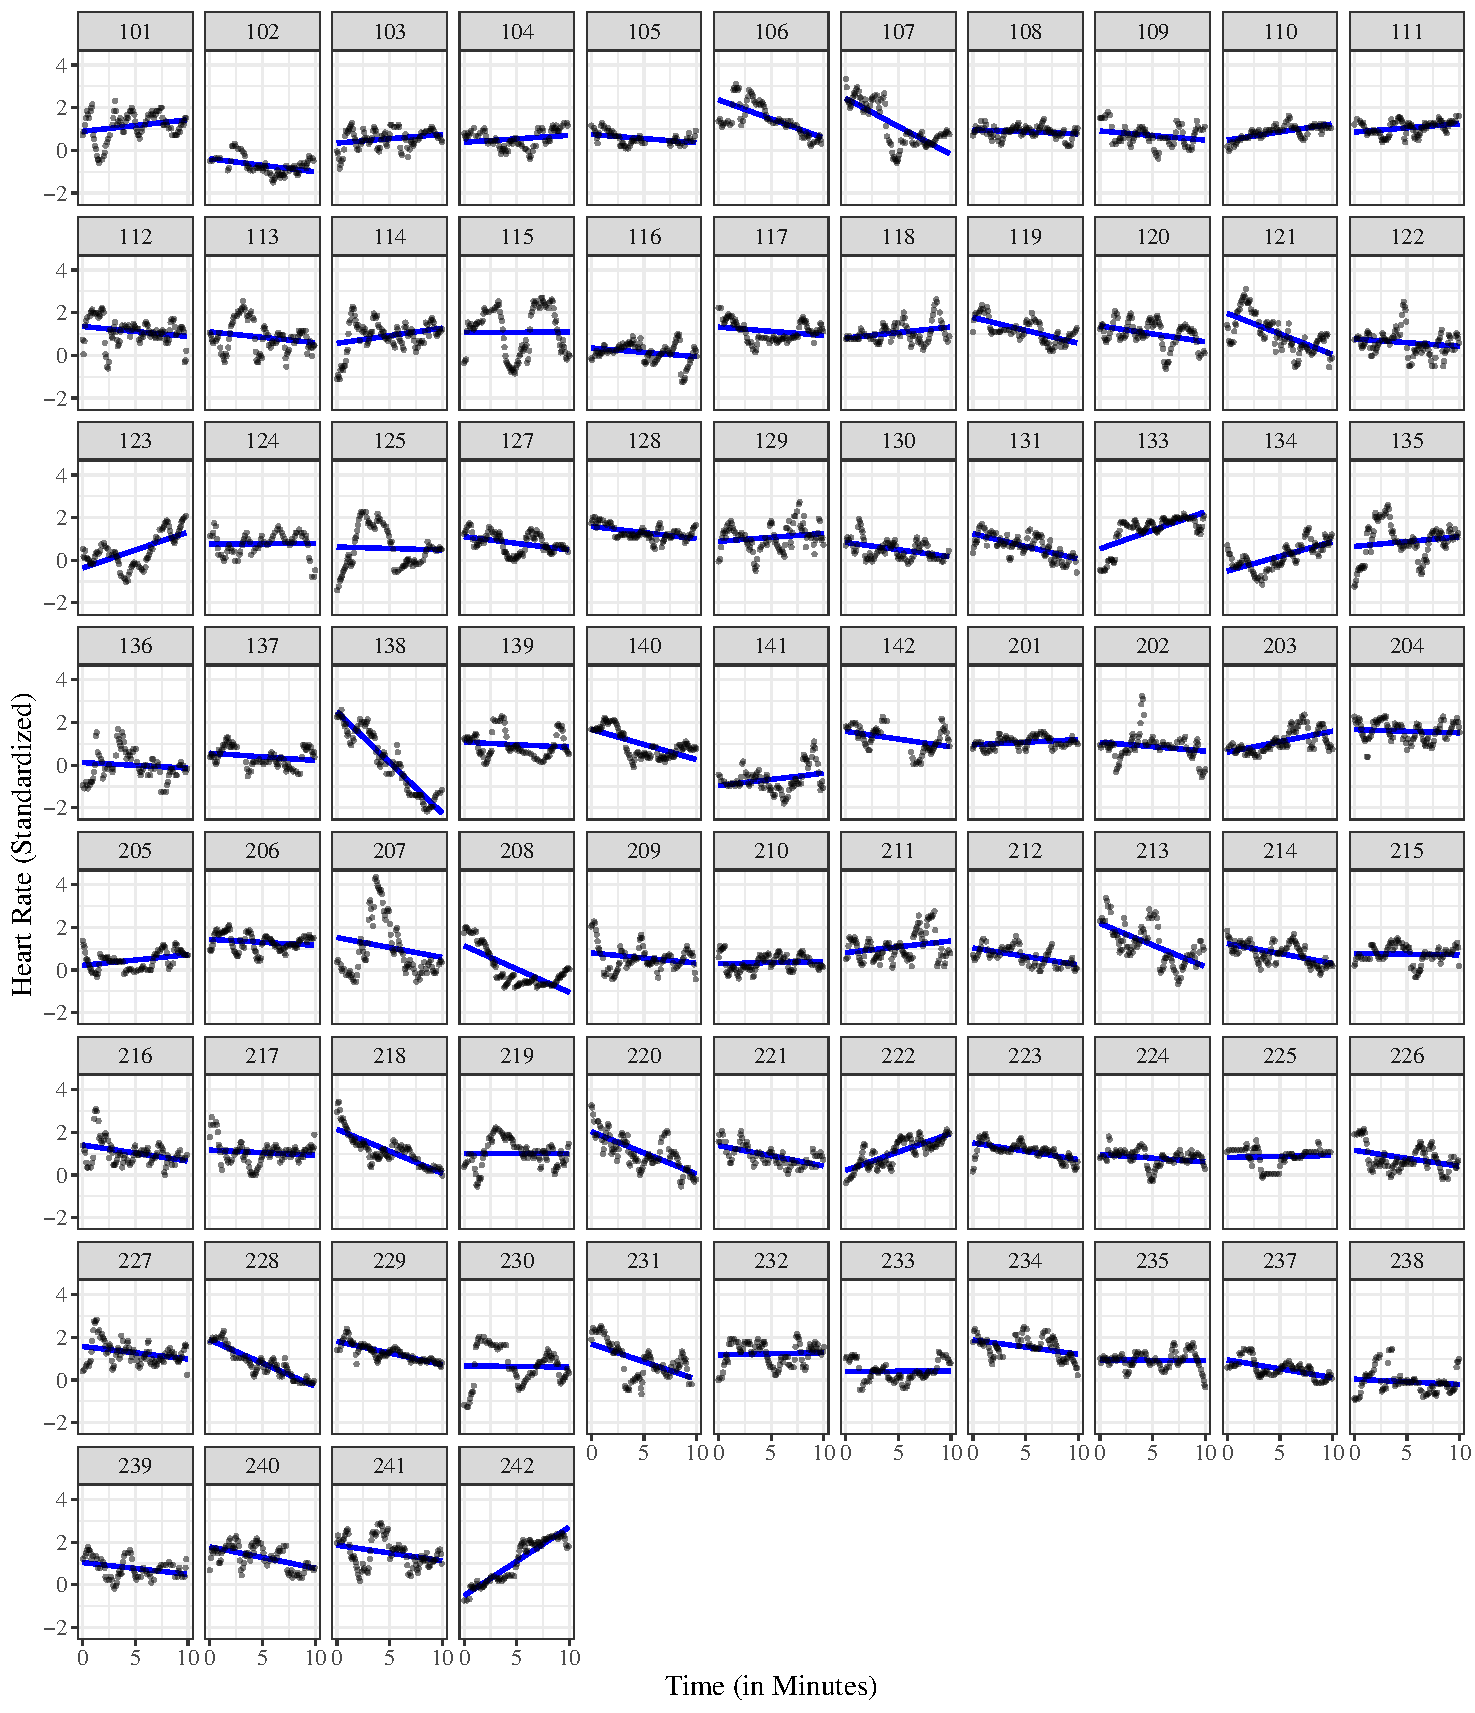
\includegraphics[width=1\textwidth]{plots_publication/plot_teaching_appendix.pdf}
  \caption{Linear estimation of individual HR changes over time during the teaching phase for $N$ = 81 participants. Each plot illustrates the mean standardized HR values (y-axis) across 10 minutes (x-axis), with the black dots representing observed HR data points and the blue line showing the estimated linear trend.}
  \label{fig.a4}
\end{figure}

\begin{figure}[htbp]
  \centering
  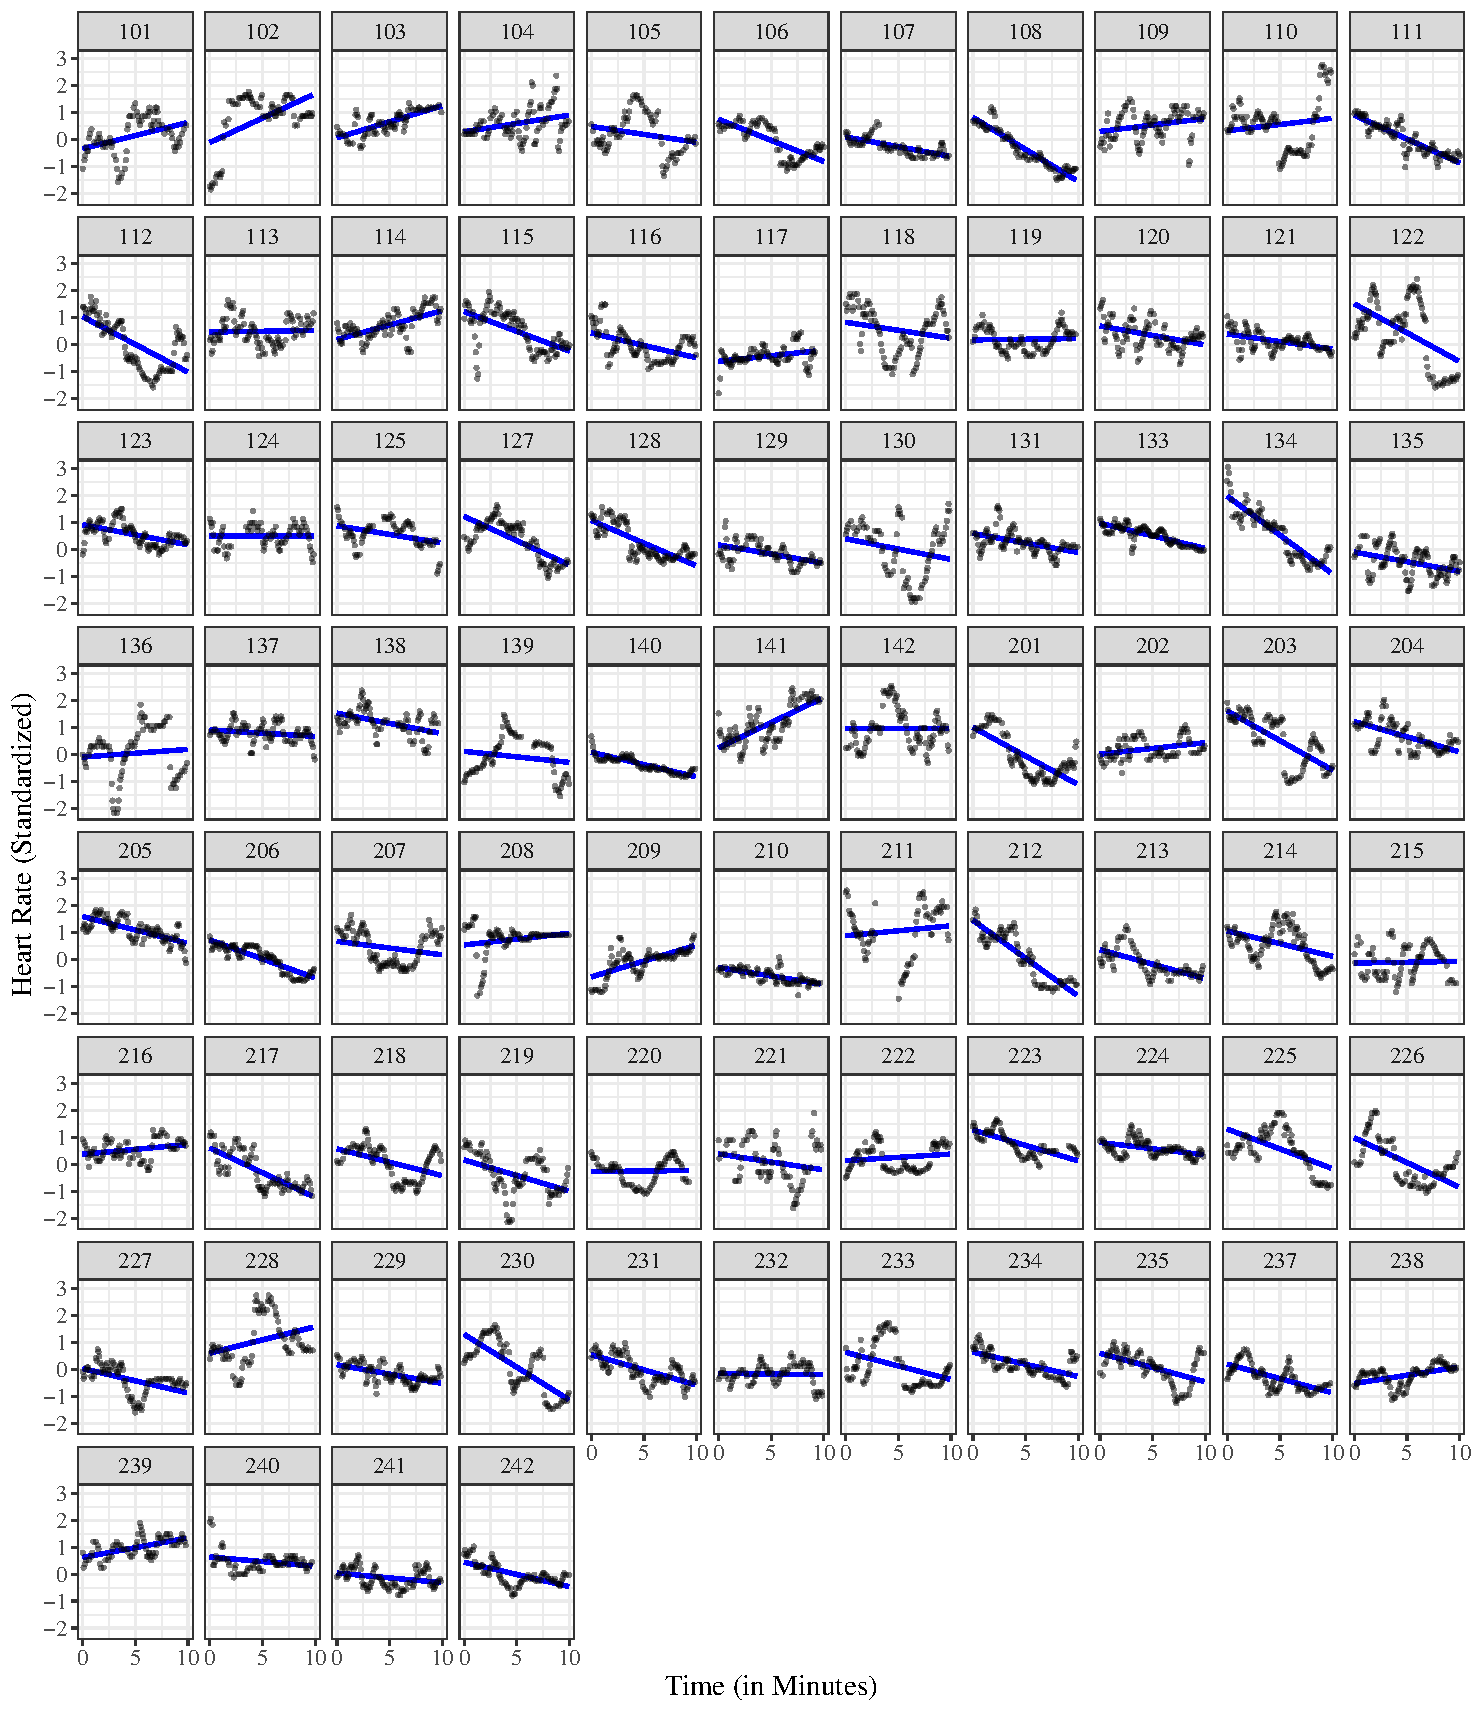
\includegraphics[width=1\textwidth]{plots_publication/plot_post_teaching_appendix.pdf}
    \caption{Linear estimation of individual HR changes over time during the post-teaching phase for $N$ = 81 participants. Each plot illustrates the mean standardized HR values (y-axis) across 10 minutes (x-axis), with the black dots representing observed HR data points and the blue line showing the estimated linear trend.}
  \label{fig.a5}
\end{figure}

\begin{figure}[htbp]
  \centering
  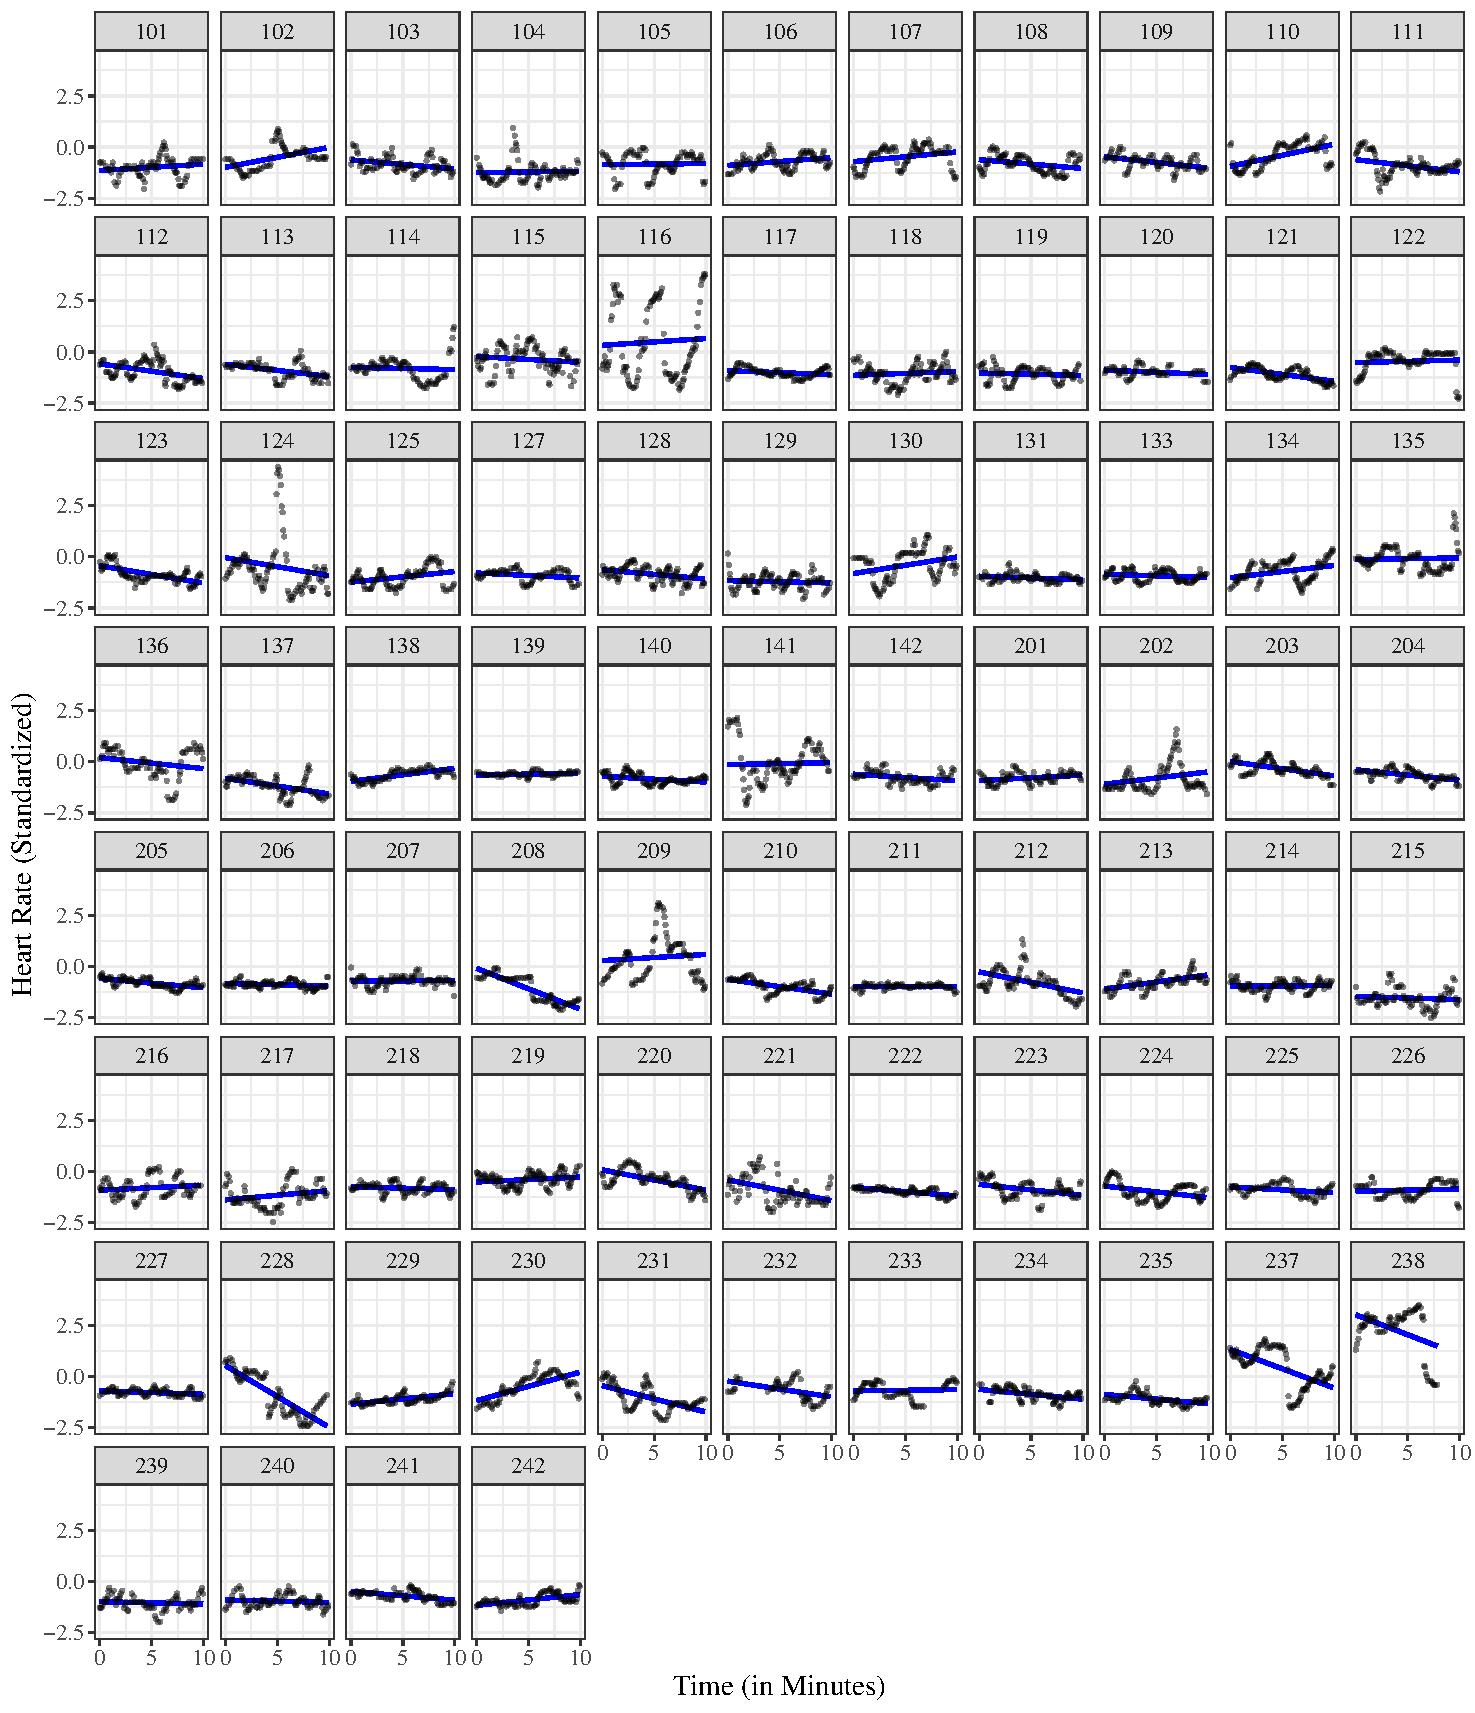
\includegraphics[width=1\textwidth]{plots_publication/plot_interview_appendix.pdf}
  \caption{Linear estimation of individual HR changes over time during the interview phase for $N$ = 81 participants. Each plot illustrates the mean standardized HR values (y-axis) across 10 minutes (x-axis), with the black dots representing observed HR data points and the blue line showing the estimated linear trend.}
  \label{fig.a6}
\end{figure}

\begin{figure}[htbp]
  \centering
  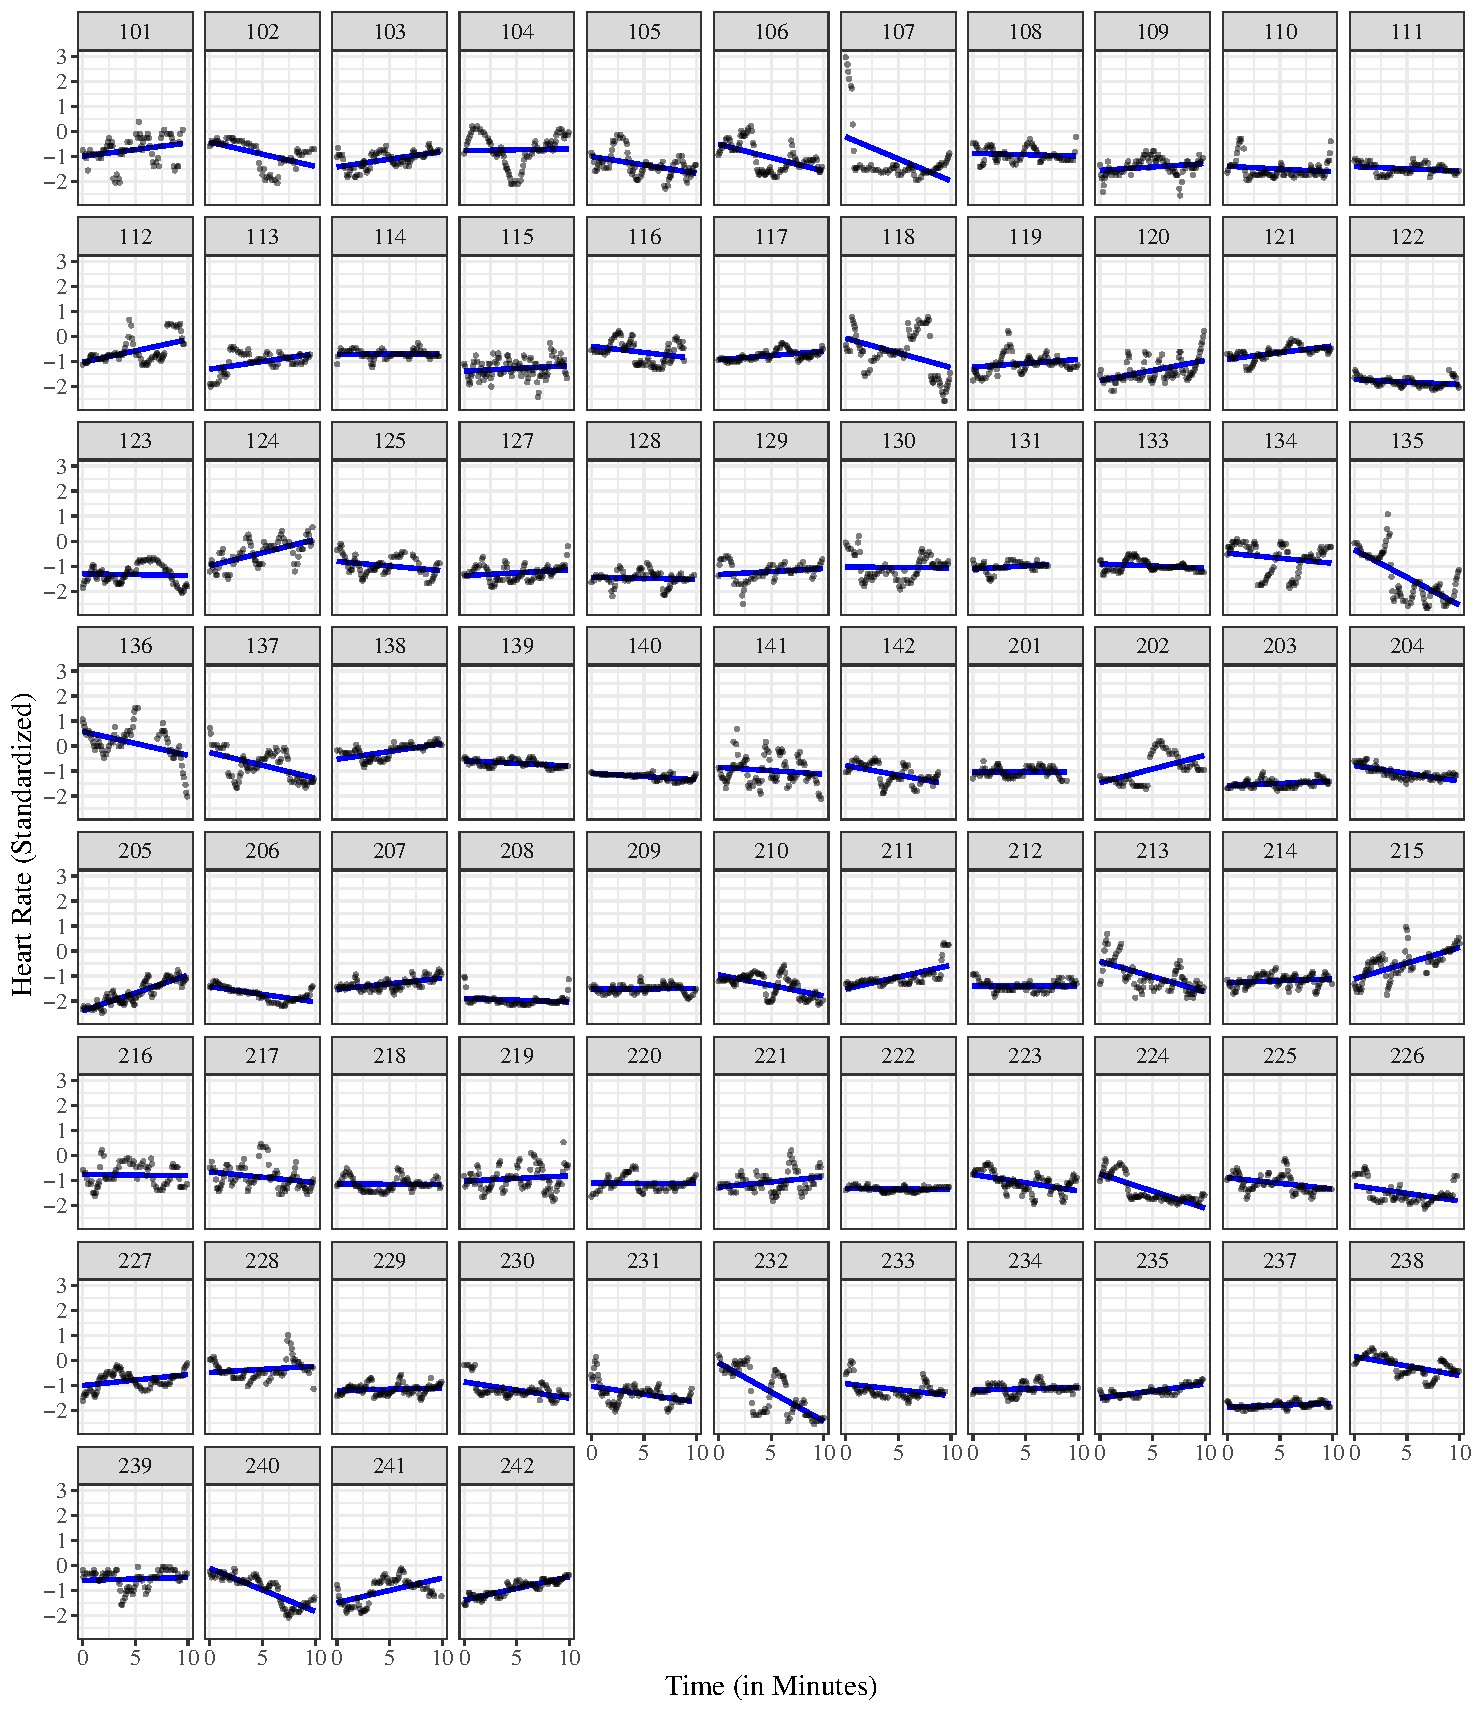
\includegraphics[width=1\textwidth]{plots_publication/plot_end_appendix.pdf}
    \caption{Linear estimation of individual HR changes over time during the end phase for $N$ = 81 participants. Each plot illustrates the mean standardized HR values (y-axis) across 10 minutes (x-axis), with the black dots representing observed HR data points and the blue line showing the estimated linear trend.}
  \label{fig.a7}
\end{figure}

\newpage

\phantomsection\label{refs}
\begin{CSLReferences}{1}{0}
\bibitem[\citeproctext]{ref-agyapong2023interventions}
Agyapong, B., P. Brett-MacLean, L. Burback, V. I. O. Agyapong, and Y.
Wei. 2023. {``Interventions to Reduce Stress and Burnout Among Teachers:
A Scoping Review.''} \emph{International Journal of Environmental
Research and Public Health} 20 (9): 5625.
\url{https://doi.org/10.3390/ijerph20095625}.

\bibitem[\citeproctext]{ref-allen2007photoplethysmography}
Allen, J. 2007. {``Photoplethysmography and Its Application in Clinical
Physiological Measurement.''} \emph{Physiological Measurement} 28 (3):
R1. \url{https://doi.org/10.1088/0967-3334/28/3/R01}.

\bibitem[\citeproctext]{ref-aloe2014multivariate}
Aloe, A. M., S. M. Shisler, B. D. Norris, A. B. Nickerson, and T. W.
Rinker. 2014. {``A Multivariate Meta-Analysis of Student Misbehavior and
Teacher Burnout.''} \emph{Educational Research Review} 12: 30--44.
\url{https://doi.org/10.1016/j.edurev.2014.05.003}.

\bibitem[\citeproctext]{ref-battipaglia2015}
Battipaglia, I., and G. A. Lanza. 2015. {``The Autonomic Nervous System
of the Heart.''} In \emph{Autonomic Innervation of the Heart: Role of
Molecular Imaging}, edited by R. H. J. A. Slart, R. A. Tio, P. H.
Elsinga, and M. Schwaiger, 1--12. Berlin, Heidelberg: Springer Berlin
Heidelberg. \url{https://doi.org/10.1007/978-3-662-45074-1_1}.

\bibitem[\citeproctext]{ref-beaty2010}
Beaty-O'Ferrall, M. E., A. Green, and F. Hanna. 2010. {``Classroom
Management Strategies for Difficult Students: Promoting Change Through
Relationships.''} \emph{Middle School Journal} 41 (4): 4--11.
\url{https://doi.org/10.2307/23044778}.

\bibitem[\citeproctext]{ref-berntson2007cardiovascular}
Berntson, G., K. Quigley, and D. Lozano. 2007. {``Cardiovascular
Psychophysiology.''} \emph{Handbook of Psychophysiology} 3: 182--210.
\url{https://doi.org/10.1017/CBO9780511546396.008}.

\bibitem[\citeproctext]{ref-boyle1995structural}
Boyle, G. J., M. G. Borg, J. M. Falzon, and A. J. Baglioni Jr. 1995.
{``A Structural Model of the Dimensions of Teacher Stress.''}
\emph{British Journal of Educational Psychology} 65 (1): 49--67.
\url{https://doi.org/10.1111/j.2044-8279.1995.tb01130.x}.

\bibitem[\citeproctext]{ref-castaneda2018review}
Castaneda, D., A. Esparza, M. Ghamari, C. Soltanpur, and H. Nazeran.
2018. {``A Review on Wearable Photoplethysmography Sensors and Their
Potential Future Applications in Health Care.''} \emph{International
Journal of Biosensors \& Bioelectronics} 4 (4): 195.
\url{https://doi.org/10.15406/ijbsbe.2018.04.00125}.

\bibitem[\citeproctext]{ref-chalmers2021}
Chalmers, T., B. A. Hickey, P. Newton, C. Lin, D. Sibbritt, C. S.
McLachlan, R. Clifton-Bligh, J. Morley, and S. Lal. 2021. {``Stress
Watch: The Use of Heart Rate and Heart Rate Variability to Detect
Stress: A Pilot Study Using Smart Watch Wearables.''} \emph{Sensors} 22
(1): 151. \url{https://doi.org/10.3390/s22010151}.

\bibitem[\citeproctext]{ref-chaplain2008}
Chaplain, R. P. 2008. {``Stress and Psychological Distress Among Trainee
Secondary Teachers in England.''} \emph{Educational Psychology} 28 (2):
195--209. \url{https://doi.org/10.1080/01443410701491858}.

\bibitem[\citeproctext]{ref-chevance2022accuracy}
Chevance, G., N. M. Golaszewski, E. Tipton, E. B. Hekler, M. Buman, G.
J. Welk, K. Patrick, J. G. Godino, et al. 2022. {``Accuracy and
Precision of Energy Expenditure, Heart Rate, and Steps Measured by
Combined-Sensing Fitbits Against Reference Measures: Systematic Review
and Meta-Analysis.''} \emph{JMIR mHealth and uHealth} 10 (4): e35626.
\url{https://doi.org/10.2196/35626}.

\bibitem[\citeproctext]{ref-claessens2017positive}
Claessens, L. C. A., J. van Tartwijk, A. C. van der Want, H. J. M.
Pennings, N. Verloop, P. J. den Brok, and T. Wubbels. 2017. {``Positive
Teacher--Student Relationships Go Beyond the Classroom, Problematic Ones
Stay Inside.''} \emph{The Journal of Educational Research} 110 (5):
478--93. \url{https://doi.org/10.1080/00220671.2015.1129595}.

\bibitem[\citeproctext]{ref-clunies2008self}
Clunies-Ross, P., E. Little, and M. Kienhuis. 2008. {``Self-Reported and
Actual Use of Proactive and Reactive Classroom Management Strategies and
Their Relationship with Teacher Stress and Student Behaviour.''}
\emph{Educational Psychology} 28 (6): 693--710.
\url{https://doi.org/10.1080/01443410802206700}.

\bibitem[\citeproctext]{ref-cohen1988statistical}
Cohen, J. 1988. {``Statistical Power for the Behavioural Sciences.
Hilsdale.''} \emph{NY: Lawrence Erlbaum} 58 (1): 7--19.

\bibitem[\citeproctext]{ref-custodis2014heart}
Custodis, F., J. C. Reil, S. H. Schirmer, O. Adam, S. Möhlenkamp, U.
Laufs, and M. Boehm. 2014. {``Heart Rate: Clinical Variable and Risk
Marker.''} \emph{Deutsche Medizinische Wochenschrift (1946)} 139 (33):
1661--68. \url{https://doi.org/10.1055/s-0034-1370223}.

\bibitem[\citeproctext]{ref-Darnell2019}
Darnell, D., and P. Krieg. 2019. {``Student Engagement, Assessed Using
Heart Rate, Shows No Reset Following Active Learning Sessions in
Lectures.''} \emph{PLoS ONE} 14.
\url{https://doi.org/10.1371/journal.pone.0225709}.

\bibitem[\citeproctext]{ref-donker2018}
Donker, M. H., T. Van Gog, and M. T. Mainhard. 2018. {``A Quantitative
Exploration of Two Teachers with Contrasting Emotions: Intra-Individual
Process Analyses of Physiology and Interpersonal Behavior.''}
\emph{Frontline Learning Research} 6 (3): 162--84.
\url{https://doi.org/10.14786/flr.v6i3.372}.

\bibitem[\citeproctext]{ref-dunn1999deliberate}
Dunn, T. G., and C. Shriner. 1999. {``Deliberate Practice in Teaching:
What Teachers Do for Self-Improvement.''} \emph{Teaching and Teacher
Education} 15 (6): 631--51.
\url{https://doi.org/10.1016/S0742-051X(98)00068-7}.

\bibitem[\citeproctext]{ref-ferguson2015}
Ferguson, T., A. V. Rowlands, T. Olds, and C. Maher. 2015. {``The
Validity of Consumer-Level, Activity Monitors in Healthy Adults Worn in
Free-Living Conditions: A Cross-Sectional Study.''} \emph{International
Journal of Behavioral Nutrition and Physical Activity} 12 (1): 1--9.
\url{https://doi.org/10.1186/s12966-015-0201-9}.

\bibitem[\citeproctext]{ref-fisher2011}
Fisher, M. H. 2011. {``Factors Influencing Stress, Burnout, and
Retention of Secondary Teachers.''} \emph{Current Issues in Education}
14 (1).

\bibitem[\citeproctext]{ref-fitbitnd}
Fitbit, Inc. 2020. \emph{Fitbit Charge 4 User Manual Version 1.2}.
Fitbit, Inc.

\bibitem[\citeproctext]{ref-fuller2020}
Fuller, D., E. Colwell, J. Low, K. Orychock, M. A. Tobin, B. Simango, R.
Buote, et al. 2020. {``Reliability and Validity of Commercially
Available Wearable Devices for Measuring Steps, Energy Expenditure, and
Heart Rate: Systematic Review.''} \emph{JMIR mHealth and uHealth} 8 (9):
e18694. \url{https://doi.org/10.2196/18694}.

\bibitem[\citeproctext]{ref-gagnon2022}
Gagnon, J., M. Khau, L. Lavoie-Hudon, F. Vachon, V. Drapeau, and S.
Tremblay. 2022. {``Comparing a Fitbit Wearable to an Electrocardiogram
Gold Standard as a Measure of Heart Rate Under Psychological Stress: A
Validation Study.''} \emph{JMIR Formative Research} 6 (12): e37885.
\url{https://doi.org/10.2196/37885}.

\bibitem[\citeproctext]{ref-gelman2006data}
Gelman, A., and J. Hill. 2006. \emph{Data Analysis Using Regression and
Multilevel/Hierarchical Models}. Cambridge university press.
\url{https://doi.org/10.1017/CBO9780511790942}.

\bibitem[\citeproctext]{ref-godfrey2018z}
Godfrey, A., V. Hetherington, H. Shum, P. Bonato, N. H. Lovell, and S.
Stuart. 2018. {``From a to z: Wearable Technology Explained.''}
\emph{Maturitas} 113: 40--47.
\url{https://doi.org/10.1016/j.maturitas.2018.04.012}.

\bibitem[\citeproctext]{ref-hajj2023}
Hajj-Boutros, G., M. Landry-Duval, A. S. Comtois, G. Gouspillou, and A.
D. Karelis. 2023. {``Wrist-Worn Devices for the Measurement of Heart
Rate and Energy Expenditure: A Validation Study for the Apple Watch 6,
Polar Vantage v and Fitbit Sense.''} \emph{European Journal of Sport
Science} 23 (2): 165--77.
\url{https://doi.org/10.1080/17461391.2021.2023656}.

\bibitem[\citeproctext]{ref-hao2018chrv}
Hao, T., H. Chang, M. Ball, K. Lin, and X. Zhu. 2017. {``cHRV Uncovering
Daily Stress Dynamics Using Bio-Signal from Consumer Wearables.''} In
\emph{MEDINFO 2017: Precision Healthcare Through Informatics}, 98--102.
IOS Press. \url{https://doi.org/10.3233/978-1-61499-830-3-98}.

\bibitem[\citeproctext]{ref-heneghan2019}
Heneghan, C., S. Venkatraman, and A. Russell. 2019. {``Investigation of
an Estimate of Daily Resting Heart Rate Using a Consumer Wearable
Device.''} \emph{medRxiv}, 19008771.
\url{https://doi.org/10.1101/19008771}.

\bibitem[\citeproctext]{ref-herman2020}
Herman, K. C., S. L. Prewett, C. L. Eddy, A. Savala, and W. M. Reinke.
2020. {``Profiles of Middle School Teacher Stress and Coping: Concurrent
and Prospective Correlates.''} \emph{Journal of School Psychology} 78:
54--68. \url{https://doi.org/10.1016/j.jsp.2019.11.003}.

\bibitem[\citeproctext]{ref-hottenrott2007}
Hottenrot, K. 2007. \emph{Trainingskontrolle: Mit
Herzfrequenz-Messgeräten, 2. Auflage}. Meyer \& Meyer Verlag.

\bibitem[\citeproctext]{ref-huang2022class}
Huang, Y., E. Richter, T. Kleickmann, and D. Richter. 2022. {``Class
Size Affects Preservice Teachers' Physiological and Psychological Stress
Reactions: An Experiment in a Virtual Reality Classroom.''}
\emph{Computers \& Education} 184: 104503.
\url{https://doi.org/10.1016/j.compedu.2022.104503}.

\bibitem[\citeproctext]{ref-ingersoll2003}
Ingersoll, R. M., and T. M. Smith. 2003. {``The Wrong Solution to the
Teacher Shortage.''} \emph{Educational Leadership} 60 (8): 30--33.

\bibitem[\citeproctext]{ref-jachymek2021}
Jachymek, M., M. T. Jachymek, R. M. Kiedrowicz, J. Kaźmierczak, E.
Płońska-Gościniak, and M. Peregud-Pogorzelska. 2021. {``Wristbands in
Home-Based Rehabilitation---Validation of Heart Rate Measurement.''}
\emph{Sensors} 22 (1): 60. \url{https://doi.org/10.3390/s22010060}.

\bibitem[\citeproctext]{ref-jalongo2006}
Jalongo, M. R., and K. Heider. 2006. {``Editorial Teacher Attrition: An
Issue of National Concern.''} \emph{Early Childhood Education Journal}
33: 379--80. \url{https://doi.org/10.1007/s10643-006-0122-y}.

\bibitem[\citeproctext]{ref-jo2016}
Jo, E., K. Lewis, D. Directo, M. J. Kim, and B. A. Dolezal. 2016.
{``Validation of Biofeedback Wearables for Photoplethysmographic Heart
Rate Tracking.''} \emph{Journal of Sports Science \& Medicine} 15 (3):
540.

\bibitem[\citeproctext]{ref-johnson2005experience}
Johnson, S., C. Cooper, S. Cartwright, I. Donald, P. Taylor, and C.
Millet. 2005. {``The Experience of Work-Related Stress Across
Occupations.''} \emph{Journal of Managerial Psychology} 20 (2): 178--87.
\url{https://doi.org/10.1108/02683940510579803}.

\bibitem[\citeproctext]{ref-junker2021}
Junker, R., M. H. Donker, and T. Mainhard. 2021. {``Potential Classroom
Stressors of Teachers: An Audiovisual and Physiological Approach.''}
\emph{Learning and Instruction} 75: 101495.
\url{https://doi.org/10.1016/j.learninstruc.2021.101495}.

\bibitem[\citeproctext]{ref-karner2021teachers}
Kärner, T., and J. Höning. 2021. {``Teachers' Experienced Classroom
Demands and Autonomic Stress Reactions: Results of a Pilot Study and
Implications for Process-Oriented Research in Vocational Education and
Training.''} \emph{Empirical Research in Vocational Education and
Training} 13: 1--22. \url{https://doi.org/10.1186/s40461-021-00113-3}.

\bibitem[\citeproctext]{ref-kirschbaum1993trier}
Kirschbaum, C., K. M. Pirke, and D. H. Hellhammer. 1993. {``The {`Trier
Social Stress Test'}--a Tool for Investigating Psychobiological Stress
Responses in a Laboratory Setting.''} \emph{Neuropsychobiology} 28
(1-2): 76--81. \url{https://doi.org/10.1159/000119004}.

\bibitem[\citeproctext]{ref-kirschner2016professionswissen}
Kirschner, S., M. Sczudlek, O. Tepner, A. Borowski, H. E. Fischer, G.
Lenske, D. Leutner, et al. 2016. {``Professionswissen in Den
Naturwissenschaften (ProwiN).''} In \emph{Entwicklung von
Professionalit{ä}t p{ä}dagogischen Personals: Interdisziplin{ä}re
Betrachtungen, Befunde Und Perspektiven}, 113--30. Springer.
\url{https://doi.org/10.1007/978-3-658-07274-2_7}.

\bibitem[\citeproctext]{ref-klusmann2012berufliche}
Klusmann, U., M. Kunter, T. Voss, and J. Baumert. 2012. {``Berufliche
Beanspruchung Angehender Lehrkr{ä}fte: Die Effekte von Pers{ö}nlichkeit,
p{ä}dagogischer Vorerfahrung Und Professioneller Kompetenz.''}
\emph{Zeitschrift f{ü}r p{ä}dagogische Psychologie}.
\url{https://doi.org/10.1024/1010-0652/a000078}.

\bibitem[\citeproctext]{ref-kranjec2014non}
Kranjec, J., S. Beguš, G. Geršak, and J. Drnovšek. 2014. {``Non-Contact
Heart Rate and Heart Rate Variability Measurements: A Review.''}
\emph{Biomedical Signal Processing and Control} 13: 102--12.
\url{https://doi.org/10.1016/j.bspc.2014.03.004}.

\bibitem[\citeproctext]{ref-kyriacou1978}
Kyriacou, C., and J. Sutcliffe. 1978. {``Teacher Stress: Prevalence,
Sources, and Symptoms.''} \emph{British Journal of Educational
Psychology} 48 (2): 159--67.
\url{https://doi.org/10.1111/j.2044-8279.1978.tb02381.x}.

\bibitem[\citeproctext]{ref-lazarus1966psychological}
Lazarus, R. S. 1966. {``Psychological Stress and the Coping Process.''}
\emph{Mc Grew-Hill}.

\bibitem[\citeproctext]{ref-lazarus1990theory}
---------. 1990. {``Theory-Based Stress Measurement.''}
\emph{Psychological Inquiry} 1 (1): 3--13.
\url{https://doi.org/10.1207/s15327965pli0101_1}.

\bibitem[\citeproctext]{ref-liu2020}
Liu, M., and Y. Yan. 2020. {``Anxiety and Stress in in-Service Chinese
University Teachers of Arts.''} \emph{International Journal of Higher
Education} 9 (1): 237--48. \url{https://doi.org/10.5430/ijhe.v9n1p237}.

\bibitem[\citeproctext]{ref-lu2008can}
Lu, S., H. Zhao, K. Ju, K. Shin, M. Lee, K. Shelley, and K. H. Chon.
2008. {``Can Photoplethysmography Variability Serve as an Alternative
Approach to Obtain Heart Rate Variability Information?''} \emph{Journal
of Clinical Monitoring and Computing} 22 (1): 23--29.
\url{https://doi.org/10.1007/s10877-007-9103-y}.

\bibitem[\citeproctext]{ref-maslach2001job}
Maslach, C., W. B. Schaufeli, and M. P. Leiter. 2001. {``Job Burnout.''}
\emph{Annual Review of Psychology} 52 (1): 397--422.
\url{https://doi.org/10.1146/annurev.psych.52.1.397}.

\bibitem[\citeproctext]{ref-montgomery2005meta}
Montgomery, C., and A. A. Rupp. 2005. {``A Meta-Analysis for Exploring
the Diverse Causes and Effects of Stress in Teachers.''} \emph{Canadian
Journal of Education/Revue Canadienne de l'{é}ducation}, 458--86.
\url{https://doi.org/10.2307/4126479}.

\bibitem[\citeproctext]{ref-montoye2017comparative}
Montoye, A. H. K., J. R. Mitrzyk, and M. J. Molesky. 2017.
{``Comparative Accuracy of a Wrist-Worn Activity Tracker and a Smart
Shirt for Physical Activity Assessment.''} \emph{Measurement in Physical
Education and Exercise Science} 21 (4): 201--11.
\url{https://doi.org/10.1080/1091367X.2017.1331166}.

\bibitem[\citeproctext]{ref-muggeridge2021measurement}
Muggeridge, D. J., K. Hickson, A. V. Davies, O. M. Giggins, I. L.
Megson, T. Gorely, and D. R. Crabtree. 2021. {``Measurement of Heart
Rate Using the Polar OH1 and Fitbit Charge 3 Wearable Devices in Healthy
Adults During Light, Moderate, Vigorous, and Sprint-Based Exercise:
Validation Study.''} \emph{JMIR mHealth and uHealth} 9 (3): e25313.
\url{https://doi.org/10.2196/25313}.

\bibitem[\citeproctext]{ref-mukhopadhyay2017wearable}
Mukhopadhyay, S. C., and T. Islam. 2017. \emph{Wearable Sensors:
Applications, Design and Implementation}. IOP Publishing.
\url{https://doi.org/10.1088/978-0-7503-1505-0}.

\bibitem[\citeproctext]{ref-nanchen2018}
Nanchen, D. 2018. {``Resting Heart Rate: What Is Normal?''}
\emph{Heart}. BMJ Publishing Group Ltd; British Cardiovascular Society.
\url{https://doi.org/10.1136/heartjnl-2017-312731}.

\bibitem[\citeproctext]{ref-nelson2020guidelines}
Nelson, B. W., C. A. Low, N. Jacobson, P. Areán, J. Torous, and N. B.
Allen. 2020. {``Guidelines for Wrist-Worn Consumer Wearable Assessment
of Heart Rate in Biobehavioral Research.''} \emph{NPJ Digital Medicine}
3 (1): 90. \url{https://doi.org/10.1038/s41746-020-0297-4}.

\bibitem[\citeproctext]{ref-nuss2021effects}
Nuss, K., K. Moore, T. Nelson, and K. Li. 2021. {``Effects of
Motivational Interviewing and Wearable Fitness Trackers on Motivation
and Physical Activity: A Systematic Review.''} \emph{American Journal of
Health Promotion} 35 (2): 226--35.
\url{https://doi.org/10.1177/0890117120939030}.

\bibitem[\citeproctext]{ref-ophardt2017klassenmanagement}
Ophardt, D., and F. Thiel. 2017. {``Klassenmanagement Als Basisdimension
Der Unterrichtsqualit{ä}t.''} \emph{Lehrer-Sch{ü}ler-Interaktion:
Inhaltsfelder, Forschungsperspektiven Und Methodische Zug{ä}nge},
245--66.

\bibitem[\citeproctext]{ref-peng2022acceptance}
Peng, C., N. Xi, H. Zhao, and J. Hamari. 2022. {``Acceptance of Wearable
Technology: A Meta-Analysis.''} In \emph{Hawaii International Conference
on System Sciences}, 5101--10.
\url{https://doi.org/10.24251/HICSS.2022.621}.

\bibitem[\citeproctext]{ref-pham2021}
Pham, T., Z. J. Lau, S. H. A. Chen, and D. Makowski. 2021. {``Heart Rate
Variability in Psychology: A Review of HRV Indices and an Analysis
Tutorial.''} \emph{Sensors} 21 (12): 3998.
\url{https://doi.org/10.3390/s21123998}.

\bibitem[\citeproctext]{ref-razavi2001self}
Razavi, T. 2001. {``Self-Report Measures: An Overview of Concerns and
Limitations of Questionnaire Use in Occupational Stress Research.''}

\bibitem[\citeproctext]{ref-ritvanen2006responses}
Ritvanen, T., V. Louhevaara, P. Helin, S. Väisänen, and O. Hänninen.
2006. {``Responses of the Autonomic Nervous System During Periods of
Perceived High and Low Work Stress in Younger and Older Female
Teachers.''} \emph{Applied Ergonomics} 37 (3): 311--18.
\url{https://doi.org/10.1016/j.apergo.2005.06.013}.

\bibitem[\citeproctext]{ref-RStudio2020}
RStudio Team. 2020. \emph{RStudio: Integrated Development Environment
for r}. Boston, MA: RStudio, PBC.

\bibitem[\citeproctext]{ref-ruedi2014}
Rüedi, J. 2014. {``Zur Bedeutung Positive Beziehungen f{ü}r Die
Klassenf{ü}hrung Und Den Umgang Mit Unterrichtsst{ö}rungen.''}
\emph{Beziehungen in Schule Und Unterricht. Teil} 3: 105--26.

\bibitem[\citeproctext]{ref-runge2020}
Runge, N., S. Haarman, and M. Fisher. 2020. {``Using Fitbit Fitness
Trackers to Measure Teacher Stress and Coping.''} \emph{International
Journal of Social Policy and Education} 2: 56--70.

\bibitem[\citeproctext]{ref-sachs2014}
Sachs, S. 2014. {``Physiologische Parameter Zur Bewertung Der
Lernwirksamkeit von Lernsituationen.''} PhD thesis, Universit{ä}t Ulm.

\bibitem[\citeproctext]{ref-sammito2015guideline}
Sammito, S., B. Thielmann, R. Seibt, A. Klussmann, M. Weippert, and I.
Böckelmann. 2015. {``Guideline for the Application of Heart Rate and
Heart Rate Variability in Occupational Medicine and Occupational
Science.''} \emph{ASU Int} 2015 (06): 1--29.
\url{https://doi.org/10.17147/ASUI.2015-06-09-03}.

\bibitem[\citeproctext]{ref-scalise2018wearables}
Scalise, L., and G. Cosoli. 2018. {``Wearables for Health and Fitness:
Measurement Characteristics and Accuracy.''} In \emph{2018 IEEE
International Instrumentation and Measurement Technology Conference
(I2MTC)}, 1--6. IEEE. \url{https://doi.org/10.1109/I2MTC.2018.8409635}.

\bibitem[\citeproctext]{ref-scheuch1997psychophysische}
Scheuch, K., and M. Knothe. 1997. {``Psychophysische Beanspruchung von
Lehrern in Der Unterrichtst{ä}tigkeit.''} \emph{Jahrbuch f{ü}r
Lehrerforschung} 1 (S 285): 299.

\bibitem[\citeproctext]{ref-schult2014belastet}
Schult, J., M. Münzer-Schrobildgen, and J. R. Sparfeldt. 2014.
{``Belastet, Aber Hochzufrieden?''} \emph{Zeitschrift f{ü}r
Gesundheitspsychologie}.
\url{https://doi.org/10.1026/0943-8149/a000114}.

\bibitem[\citeproctext]{ref-smith2000}
Smith, A. 2000. {``The Scale of Perceived Occupational Stress.''}
\emph{Occupational Medicine} 50 (5): 294--98.
\url{https://doi.org/10.1093/occmed/50.5.294}.

\bibitem[\citeproctext]{ref-sperka1995}
Sperka, M., and U.. Kittler. 1995. {``Psychophysiologische Beanspruchung
von Lehramtskandidatinnen Und -Kandidaten Im Schulunterricht.''} In
\emph{Psychische Potentiale Für Eine Interdisziplinäre Lehrerausbildung:
Motivation - Kognition -- Entwicklung}, edited by K. Bräuer, 182--97.
Essen: Die Blaue Eule.

\bibitem[\citeproctext]{ref-taelman2009influence}
Taelman, J., S. Vandeput, A. Spaepen, and S. Van Huffel. 2009.
{``Influence of Mental Stress on Heart Rate and Heart Rate
Variability.''} In \emph{4th European Conference of the International
Federation for Medical and Biological Engineering}, 1366--69. Springer.
\url{https://doi.org/10.1007/978-3-540-89208-3_324}.

\bibitem[\citeproctext]{ref-thomson2019heart}
Thomson, E. A., K. Nuss, A. Comstock, S. Reinwald, S. Blake, R. E.
Pimentel, B. L. Tracy, and K. Li. 2019. {``Heart Rate Measures from the
Apple Watch, Fitbit Charge HR 2, and Electrocardiogram Across Different
Exercise Intensities.''} \emph{Journal of Sports Sciences} 37 (12):
1411--19. \url{https://doi.org/10.1080/02640414.2018.1560644}.

\bibitem[\citeproctext]{ref-trull2013ambulatory}
Trull, T. J., and U. Ebner-Priemer. 2013. {``Ambulatory Assessment.''}
\emph{Annual Review of Clinical Psychology} 9 (1): 151--76.
\url{https://doi.org/10.1146/annurev-clinpsy-050212-185510}.

\bibitem[\citeproctext]{ref-uchino2010older}
Uchino, B. N., W. Birmingham, and C. A. Berg. 2010. {``Are Older Adults
Less or More Physiologically Reactive? A Meta-Analysis of Age-Related
Differences in Cardiovascular Reactivity to Laboratory Tasks.''}
\emph{Journals of Gerontology Series B: Psychological Sciences and
Social Sciences} 65 (2): 154--62.
\url{https://doi.org/10.1093/geronb/gbp127}.

\bibitem[\citeproctext]{ref-unterbrink2007}
Unterbrink, T., A. Hack, R. Pfeifer, V. Buhl-Grießhaber, U. Müller, H.
Wesche, M. Frommhold, et al. 2007. {``Burnout and
Effort--Reward-Imbalance in a Sample of 949 German Teachers.''}
\emph{International Archives of Occupational and Environmental Health}
80: 433--41. \url{https://doi.org/10.1007/s00420-007-0169-0}.

\bibitem[\citeproctext]{ref-van2016accuracy}
Van den Bergh, O., and M. Walentynowicz. 2016. {``Accuracy and Bias in
Retrospective Symptom Reporting.''} \emph{Current Opinion in Psychiatry}
29 (5): 302--8. \url{https://doi.org/10.1097/YCO.0000000000000267}.

\bibitem[\citeproctext]{ref-van2006stress}
Van Dick, R. 2006. {``Stress Und Arbeitszufriedenheit Bei Lehrerinnen
Und Lehrern.''} \emph{Zwischen „Horrorjob ``Und Erf{ü}llung} 2.

\bibitem[\citeproctext]{ref-wallen2016accuracy}
Wallen, M. P., S. R. Gomersall, S. E. Keating, U. Wisløff, and J. S.
Coombes. 2016. {``Accuracy of Heart Rate Watches: Implications for
Weight Management.''} \emph{PloS One} 11 (5): e0154420.
\url{https://doi.org/10.1371/journal.pone.0154420}.

\bibitem[\citeproctext]{ref-wettstein2020ambulatory}
Wettstein, A., F. Kühne, W. Tschacher, and R. La Marca. 2020.
{``Ambulatory Assessment of Psychological and Physiological Stress on
Workdays and Free Days Among Teachers. A Preliminary Study.''}
\emph{Frontiers in Neuroscience} 14: 495378.
\url{https://doi.org/10.3389/fnins.2020.00112}.

\bibitem[\citeproctext]{ref-wettstein2021}
Wettstein, A., S. Schneider, M. Grosse Holtforth, and R. La Marca. 2021.
{``Teacher {Stress}: {A} {Psychobiological} {Approach} to {Stressful}
{Interactions} in the {Classroom}.''} \emph{Frontiers in Education} 6.
\url{https://doi.org/10.3389/feduc.2021.681258}.

\bibitem[\citeproctext]{ref-ggplot2}
Wickham, H. 2016. \emph{Ggplot2: Elegant Graphics for Data Analysis}.
Springer-Verlag New York.
\url{https://doi.org/10.1007/978-0-387-98141-3}.

\bibitem[\citeproctext]{ref-wolff2015keeping}
Wolff, C. E., N. van den Bogert, H. Jarodzka, and H. P. A. Boshuizen.
2015. {``Keeping an Eye on Learning: Differences Between Expert and
Novice Teachers' Representations of Classroom Management Events.''}
\emph{Journal of Teacher Education} 66 (1): 68--85.
\url{https://doi.org/10.1177/0022487114549810}.

\bibitem[\citeproctext]{ref-wolff2021classroom}
Wolff, C. E., H. Jarodzka, and H. P. A. Boshuizen. 2021. {``Classroom
Management Scripts: A Theoretical Model Contrasting Expert and Novice
Teachers' Knowledge and Awareness of Classroom Events.''}
\emph{Educational Psychology Review} 33 (1): 131--48.
\url{https://doi.org/10.1007/s10648-020-09542-0}.

\end{CSLReferences}


\end{document}
